\documentclass[11pt,a4paper,titlepage,twoside,openright]{report}
\usepackage[utf8]{inputenc}
\usepackage[T1]{fontenc}
\usepackage[spanish]{babel}
\usepackage[dvips]{graphicx}
\usepackage[nottoc,numbib]{tocbibind}
\usepackage{alltt}
\usepackage{amsmath}
\usepackage{amssymb}
\usepackage{color}
\usepackage{enumitem}
\usepackage{epsfig}
\usepackage{eurosym}
\usepackage{fancyhdr}
\usepackage{float}
\usepackage{graphics}
\usepackage{lettrine}
\usepackage{longtable}
\usepackage{mathpazo}
\usepackage[scaled=1.01]{inconsolata}
\usepackage{moreverb}
\usepackage{multirow}
\usepackage{pdfpages}
\usepackage{rotating}
\usepackage{sectsty}
\usepackage{subfigure}
\usepackage{tabu}
\usepackage{tabularx}
\usepackage{url}
\usepackage[hidelinks,pdftex,
            pdfauthor={Author Name},
            pdftitle={Project Title},
            pdfsubject={Trabajo de Fin de Grado},
            pdfkeywords={},
            pdfproducer={LaTeX},
            pdfcreator={pdflatex}]{hyperref}

\pagestyle{headings}

\setlength{\textwidth}{14.5cm}
\setlength{\textheight}{19.5cm}
\setlength{\oddsidemargin}{0.96cm}
\setlength{\evensidemargin}{0.46cm}
\setlength{\topmargin}{1.46cm}
\setlength{\footskip}{0.7cm}

\definecolor{udcpink}{RGB}{177,0,114}
\definecolor{udcgray}{RGB}{100,100,100}
\definecolor{irlabpink}{RGB}{241,92,135}
\definecolor{irlabblue}{RGB}{239,248,255}

%Doble espaciado
\renewcommand{\baselinestretch}{1.1}
\setlength{\parskip}{3pt}
\renewcommand*{\arraystretch}{1}

\hyphenation{Map-Reduce}
\hyphenation{shuffle}

% Title Page
\title{This is my title}
\author{I am the author}
\begin{document}
\def\tablename{Tabla}
\def\listtablename{Índice de Tablas}
\def\listfigurename{Índice de Figuras}

%%%%%%%%%%%%%%%%%%%%%%%%%%%%%%%%%%%%%%%%
% Portada
%%%%%%%%%%%%%%%%%%%%%%%%%%%%%%%%%%%%%%%%
\begin{titlepage}

\begin{center}
\hspace{36.5pt}\textcolor{udcgray}{{\fontfamily{phv}\selectfont Departamento de Computación}}\\\vspace{-2pt}
\hspace{4pt}\textcolor{udcpink}{{\fontfamily{phv}\selectfont Facultade de Informática}}\\\vspace{-5pt}

\includegraphics[scale=0.3]{img/udc}\\[35pt]
{\large TRABALLO DE FIN DE GRADO \\ GRADO EN ENXEÑERÍA INFORMÁTICA\\Mención en Sistemas de Información}\\[50pt]
\textbf{\begin{huge}Aplicación móvil para actividades a campo abierto\end{huge}
}\\[150pt]
\end{center}

\vspace{2cm}

\begin{flushright}
 \begin{tabular}{ll}
{\large {\bf Alumno:}}  & {\large Alberto Ramil Fernández}\\
{\large {\bf Directores:}} & {\large Javier Parapar López}\\
& {\large  Óscar Pedreira Fernández} \\
\end{tabular}\\
\vspace{0.5cm}
 {\large A Coruña, \today}
\end{flushright}

\end{titlepage}
\pagestyle{empty}
\cleardoublepage


%%%%%%%%%%%%%%%%%%%%%%%%%%%%%%%%%%%%%%%%
% Datos del trabajo
%%%%%%%%%%%%%%%%%%%%%%%%%%%%%%%%%%%%%%%%
\begin{titlepage}
\begin{Huge}{\bf Datos del trabajo}\end{Huge}\\
\newline

\begin{tabularx}{\textwidth}{XX}
\hline
{\large {\bf Título del Trabajo:}} & {\large Aplicación móvil para }\\
	& {\large actividades a campo abierto}\\
& \\
{\large {\bf Clase a la que pertenece:}} & {\large Trabajo Clásico de Ingeniería}\\
& \\
{\large {\bf Alumno:}}  & {\large Alberto Ramil Fernández }\\
& \\
{\large {\bf Directores:}} &{\large Javier Parapar López} \\
 &{\large Óscar Pedreira Fernández} \\\hline
\end{tabularx}

\vspace{1cm}

\begin{tabularx}{\textwidth}{ll}
\hline
{\large {\bf Miembros del tribunal:}}\\
\\
\\
\\
\\
\\
\\ \hline
\end{tabularx}

\vspace{1cm}

\begin{tabularx}{\textwidth}{XX}
\hline
{\large {\bf Fecha de lectura y defensa:}} & {\large A Coruña, \today}\\
\hline
\end{tabularx}

\vspace{1cm}

\begin{tabularx}{\textwidth}{XX}
\hline
{\large {\bf Calificación:}} & \\
\hline
\end{tabularx}

\end{titlepage}
\cleardoublepage


%%%%%%%%%%%%%%%%%%%%%%%%%%%%%%%%%%%%%%%%
% Certifico
%%%%%%%%%%%%%%%%%%%%%%%%%%%%%%%%%%%%%%%%
\begin{titlepage}
\pagestyle{empty}

\begin{minipage}[t][4cm][l]{.4\textwidth}
\begin{center}
{\sc Javier Parapar López}

Profesor de Universidad

Departamento de Computación

Universidade da Coruña
\end{center}
\end{minipage}
\begin{minipage}[t][4cm][l]{.1\textwidth}
\begin{center}
\vspace{1.2\baselineskip}
y
\end{center}
\end{minipage}
\begin{minipage}[t][4cm][l]{.4\textwidth}
\begin{center}
{\sc Óscar Pedreira Fernández}

Profesor de Universidad

Departamento de Computación

Universidade da Coruña
\end{center}
\end{minipage}

\vspace{2cm}

CERTIFICAN:
Que la memoria titulada {\it Aplicación móvil para actividades a campo abierto} ha sido realizada por {\sc Alberto Ramil Fernández} bajo su dirección y constituye su Traballo de Fin de Grado en el Grado de Enxeñería Informática.\\[4pt]
\begin{center}
En A Coruña, a \today
\end{center}

\vspace{3cm}

\begin{minipage}[t][5cm][l]{.45\textwidth}
\begin{center}
{\sc Javier Parapar López}

Director
\end{center}
\end{minipage}
\begin{minipage}[t][5cm][l]{.45\textwidth}
\begin{center}
{\sc Óscar Pedreira Fernández}

Director
\end{center}
\end{minipage}
\end{titlepage}
\cleardoublepage


%%%%%%%%%%%%%%%%%%%%%%%%%%%%%%%%%%%%%%%%
% Dedicatoria
%%%%%%%%%%%%%%%%%%%%%%%%%%%%%%%%%%%%%%%%
\begin{titlepage}
\vspace*{\stretch{1}}
\hfill \emph{Dedicatoria}
\vspace*{\stretch{1}}
\end{titlepage}
\cleardoublepage


%%%%%%%%%%%%%%%%%%%%%%%%%%%%%%%%%%%%%%%%
% Agradecimientos
%%%%%%%%%%%%%%%%%%%%%%%%%%%%%%%%%%%%%%%%
\begin{titlepage}
\vspace{2cm}
\begin{Huge}{\bf Agradecimientos}\end{Huge}\\
\newline


{\it
 A los profesores y ya amigos Javier Parapar López y Óscar Pedreira Fernández por su paciencia y ayuda a lo largo de este proyecto. Y que junto a Daniel Varcarce hicieron que cambiara mi rumbo en la carrera.\\
A mis padres por su paciencia.\\
A mis hermanos Rufo y Jara por aguantarme los fines de semana.\\
Y Arturo por su ayuda.
}
\\ 

\normalfont
\vspace{1cm}
\hfill{Alberto Ramón Ramil Fernández}

\hfill{A Coruña, \today}

\end{titlepage}
\cleardoublepage


%%%%%%%%%%%%%%%%%%%%%%%%%%%%%%%%%%%%%%%%
% Resumen
%%%%%%%%%%%%%%%%%%%%%%%%%%%%%%%%%%%%%%%%
\begin{titlepage}
\vspace{2cm}
\begin{Huge}{\bf Resumen}\end{Huge}\\
\newline
	El uso de dispositivos móviles en la vida cotidiana se ha ido incrementando exponencialmente en los últimos años. Como parte de esta tendencia, el uso de los dispositivos móviles se ha extendido a actividades como de ocio como al aire libre, como la pesca o la caza. En estas actividades, normalmente se necesita recordar puntos clave para poder volver a visitarlos en otras ocasiones, o las rutas seguidas para llegar a los mismos. Normalmente estas actividades se realizan en lugares de difícil acceso y un tanto peligrosos, bien por la peligrosa orografía de los accesos como del lugar en si mismo donde se practica.\\

Estos motivos nos llevaron a proponer este Trabajo de Fin de Grado.\\


El objetivo es desarrollar una aplicación móvil Android que permita al usuario realizar un seguimiento de sus jornadas tanto de caza como de pesca  y que le permita guardar sus puntos destacados para poder visitarlos en otras ocasiones. Además, la aplicación permitirá salidas en grupo, en las que cada usuario conocerá la posición de lo demás en todo momento. Poder monitorizar las jornadas conjuntamente siempre es un punto a favor en cuanto a la seguridad en estas actividades.\\



 La aplicación contará con una parte cliente(la propia aplicación nativa Android) y una parte servidor. La aplicación Android será la interfaz con la que que interactuará el usuario y en la que podrá visualizar toda la información. La parte servidora se encargará de almacenar los datos de forma persistente y de implementar los casos de uso. La comunicación entre ambas partes de llevará a cabo mediante servicios Web. En la aplicación móvil usaremos otros servicios propios de Android como Google Maps, Firebase y Location.\\



El proyecto seguirá la metodología ágil Scrum, que hará que éste esté dividido en una serie de Sprints. En cada Sprint  se llevarán a cabo trabajos de análisis, planificación, diseño, implementación y pruebas.\\

Todo lo anteriormente mencionado será recogido en esta memoria y comentado más profundamente.







\end{titlepage}
\cleardoublepage


%%%%%%%%%%%%%%%%%%%%%%%%%%%%%%%%%%%%%%%%
% Palabras clave
%%%%%%%%%%%%%%%%%%%%%%%%%%%%%%%%%%%%%%%%
\begin{titlepage}
\vspace{2cm}
\begin{Huge}{\bf Palabras clave}\end{Huge}\\
\newline

\begin{tabular}{c}
\hspace{10cm} \ \\
\end{tabular}\\
{\small \textsc{ First keyword, second keyword, etc.}}\\
\end{titlepage}
\cleardoublepage


%%%%%%%%%%%%%%%%%%%%%%%%%%%%%%%%%%%%%%%%
% Page style
%%%%%%%%%%%%%%%%%%%%%%%%%%%%%%%%%%%%%%%%
\pagestyle{fancy}
\renewcommand{\chaptermark}[1]{\markboth{
	 \MakeUppercase{\chaptername}\ \thechapter.\ \\ {\scriptsize #1}}{}}
\renewcommand{\sectionmark}[1]{\markright{
	 {\scriptsize \thesection\  #1}}{}}

\makeatletter
\def\cleardoublepage{\clearpage\if@twoside \ifodd\c@page\else
  \hbox{}\thispagestyle{empty}\newpage\if@twocolumn\hbox{}\newpage\fi\fi\fi}
\makeatother

%%%%%%%%%%%%%%%%%%%%%%%%%%%%%%%%%%%%%%%%
% Índice
%%%%%%%%%%%%%%%%%%%%%%%%%%%%%%%%%%%%%%%%
\tableofcontents


%%%%%%%%%%%%%%%%%%%%%%%%%%%%%%%%%%%%%%%%
% Capítulos
%%%%%%%%%%%%%%%%%%%%%%%%%%%%%%%%%%%%%%%%
\chapter{Introducción}
        \label{intro}
        En este primer capítulo de esta memoria se comentaran la motivación, los objetivos de la aplicación y la estructura de esta memoria. 
\section{Motivación}
Dado el creciente uso de los dispositivos móviles en los deportes al aire libre, como en caza y pesca, se aprecia una creciente demanda de aplicaciones que permitan el registro de estas actividades.\\

Uno de los aspectos más importantes de este tipo de actividades es la seguridad. Durante las jornadas de caza los cazadores caminan por el monte en grupos. Esto puede producir que en determinados momentos un cazador no conozca la situación de sus compañeros.
Esta aplicación permitirá conocer la ubicación de cada cazador en todo momento pudiendo minimizar accidentes por disparos fortuitos. Las jornadas de pesca en ocasiones  se realizan desde acantilados o lugares muy lejos de carreteras. Esto lleva a que, si tenemos una pequeña lesión, indicar nuestra ubicación a nuestros compañeros sea de gran ayuda.

Según datos del Consejo Superior de Deportes, en España  se tramitaron en el año 2016 343.130 licencias federativas de caza y 54.992 licencias de pesca. A estas personas son a las que iría dirigida esta aplicación. Cabe destacar que existen tanto cazadores como pescadores que realizan sus actividades sin tener que estar federados, por lo que el número de licencias federativas aumentaría. 





Por todo esto se propone este Trabajo de Fin de Grado.
El objetivo de este proyecto será diseñar y construir una herramienta que permita gestionar las actividades a campo abierto como
caza y pesca, permitiendo mediante geolocalización guardar los puntos de interés, las rutas seguidas,
llevar control de los usuarios presentes, guardar información de los éxitos de las jornadas y poder realizar jornadas de caza y pesca con un seguimiento  total de nuestros compañeros.


\section{Objetivos}
El objetivo es desarrollar una aplicación móvil en Android que permita al usuario realizar un seguimiento de sus jornadas tanto de caza como de pesca  y que le permita guardar sus puntos destacados para poder visitarlos en otras ocasiones. Sin olvidar que el poder monitorizar la jornadas conjuntamente siempre es un punto a favor para seguridad de los participantes en estas actividades.\\ 
Los principales objetivos serán:

\begin{itemize}
\item Registro de usuarios y adición de amigos a usuario.
\item El usuario podrá conocer su ubicación en tiempo real en un mapa.
\item El usuario podrá comenzar y parar una jornada.
\item El usuario podrá visualizar la ruta seguida durante la jornada.
\item Administrar puntos clave para el usuario.
\item Clasificación de los puntos de interés según su tipología.
\item Visualizar dichos puntos en un mapa.
\item Gestionar grupos de usuarios participantes en la jornada y poder ver su ubicación en tiempo
real.

\end{itemize}


\section{Estructura de la memoria}
La memoria del presente proyecto está estructurada del siguiente modo:

\begin{itemize}
\item \textbf{Introducción.} Contextualiza el proyecto, introduce el tema a tratar y detalla los objetivos del mismo desde un punto de vista global.
 También comenta la estructura de la memoria.

\item \textbf{Tecnología.} Describe y justifica las principales tecnologías empleadas para desarrollar el proyecto.



\item \textbf{Proceso de ingeniería.} Detallamos el proceso de ingeniería: la metodología empleada,como funciona, la adaptación de la misma y los participantes.


\item \textbf{Análisis.} Comentamos las funcionalidades de la aplicación, describiendo más detenidamente los casos de uso y requisitos. 
\item \textbf{Seguimiento.} Comentamos las fases que pasa el proyecto usando la metodología Scrum.
\item \textbf{Diseño.} Describimos la arquitectura del proyecto.
\item \textbf{Implementación.} Describiremos aspectos concretos destacados de la implementación y las pruebas realizadas.





\item \textbf{Conclusiones y trabajo futuro}
Comentamos el producto obtenido y futuros cambios que se podrían realizar.



\end{itemize}

\section{Estudio de mercado}
En esta sección comentaremos otras aplicaciones que presentan funcionalidades similares a las de este trabajo de fin de grado.



\subsection{iHunt Journal}

iHunt Journal es una aplicación de software de cacería que presenta las siguientes características: 
\begin{itemize}
\item Ver puntos en el mapa, figura \ref{fig:iHunt1}
\item Guardar puntos en un mapa,figura \ref{fig:iHunt2}
\item Puede grabar sus búsquedas.
\item Graba  estadísticas.
\item Permite planificar las próximas cacerías según meteorología, figura \ref{fig:iHunt3}.
\item Puede grabar sus trofeos figura \ref{fig:iHunt4}.

\end{itemize}

\begin{figure}[htbp]
\begin{minipage}[b]{0.5\linewidth} %Una minipágina que cubre la mitad de la página
\centering
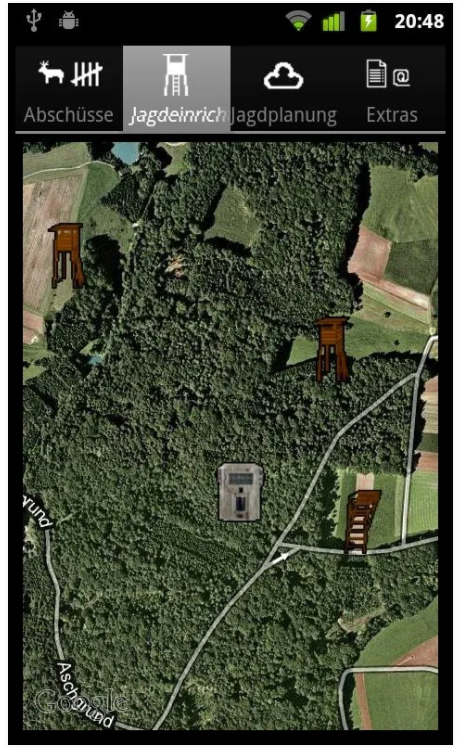
\includegraphics[width=6cm]{iHunt1.png}
\caption{ Visualizar mapa con iHunt}
\label{fig:iHunt1}
\end{minipage}
\hspace{0.5cm} % Si queremos tener un poco de espacio entre las dos figuras
\begin{minipage}[b]{0.5\linewidth}
\centering
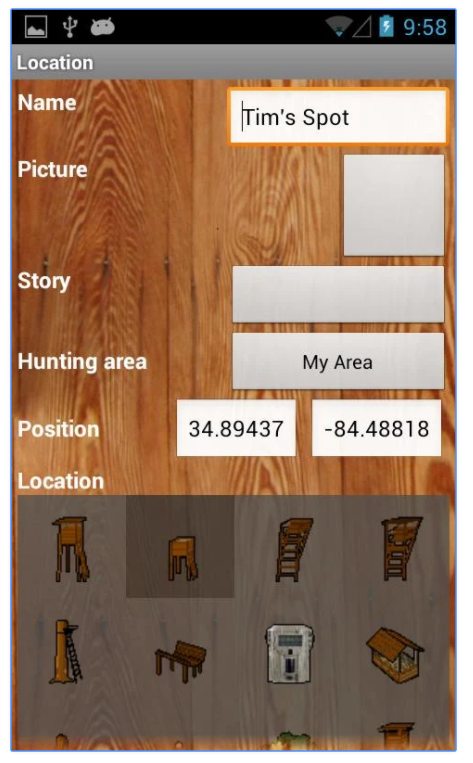
\includegraphics[width=6cm]{iHunt2.png}

\caption{Registro de un punto con iHunt}
\label{fig:iHunt2}
\end{minipage}
\begin{minipage}[b]{0.5\linewidth}
\centering
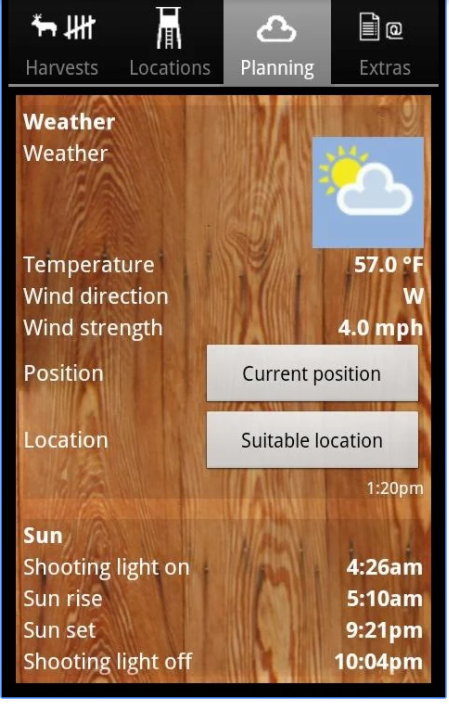
\includegraphics[width=6cm]{iHunt3.png}

\caption{Planificación con iHunt}
\label{fig:iHunt3}
\end{minipage}
\begin{minipage}[b]{0.5\linewidth}
\centering
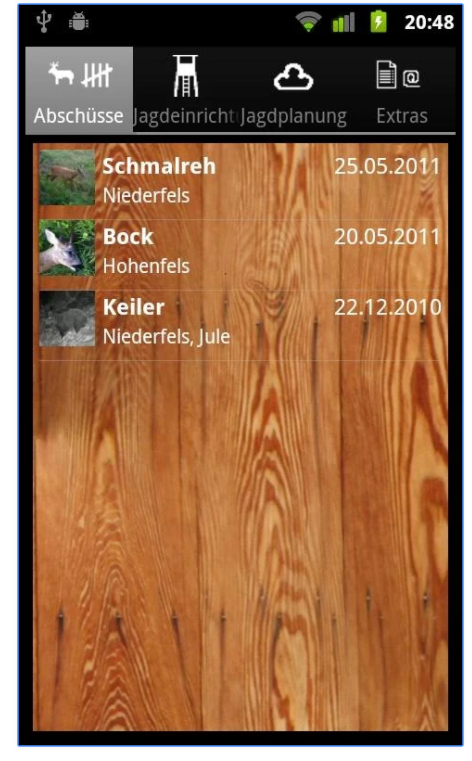
\includegraphics[width=6cm]{iHunt4.png}

\caption{Registro de trofeo con iHunt}
\label{fig:iHunt4}
\end{minipage}
\end{figure}

iHunt Journal está disponible desde iPhone y Android .


\subsection{My Fishing Companion}
 My Fishing Companion se trata de una aplicación para salir de pesca para Smartphone Android. Nos da la posibilidad de:
\begin{itemize}
\item Localizar nuestros lugares de capturas  véase figura \ref{fig:pesca2}
 \item Añadir vídeos y fotos
 \item 	Ver el tiempo que nos espera véase figura \ref{fig:pesca4}
  \item  Marcar capturas  véase figura \ref{fig:pesca3}
\end{itemize} 
 
 
 También es interesante la comunidad en la que se comparten todos estos datos y que te pueden ayudar a elegir el mejor lugar y el mejor día de pesca.
 
 \begin{figure}[htbp]
\begin{minipage}[b]{0.5\linewidth} %Una minipágina que cubre la mitad de la página
\centering
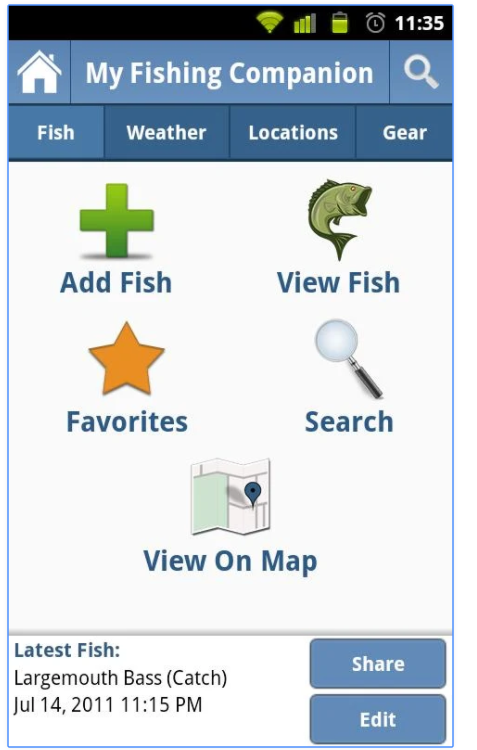
\includegraphics[width=6cm]{pesca1.png}
\caption{ Opciones de la aplicación}
\label{fig:pesca1}
\end{minipage}
\hspace{0.5cm} % Si queremos tener un poco de espacio entre las dos figuras
\begin{minipage}[b]{0.5\linewidth}
\centering
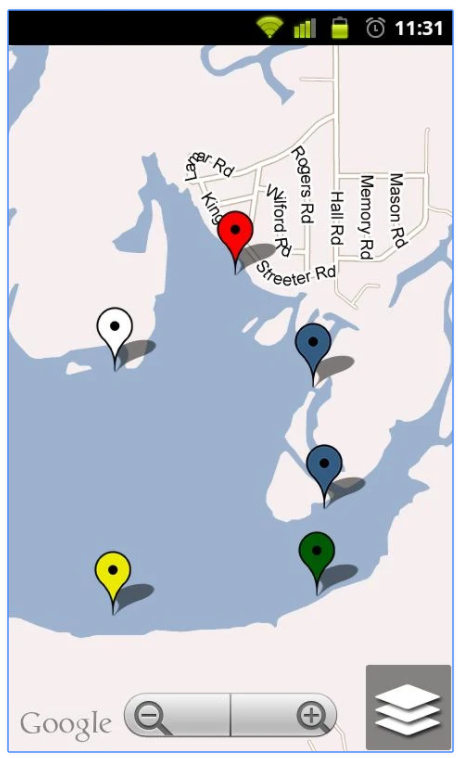
\includegraphics[width=6cm]{pesca2.png}

\caption{Puntos de pesca guardados}
\label{fig:pesca2}
\end{minipage}
\begin{minipage}[b]{0.5\linewidth}
\centering
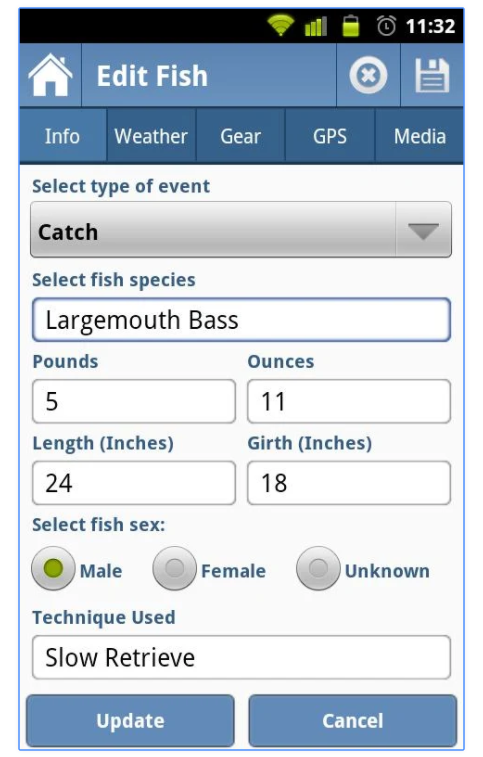
\includegraphics[width=6cm]{pesca3.png}

\caption{Datos de una captura}
\label{fig:pesca3}
\end{minipage}
\begin{minipage}[b]{0.5\linewidth}
\centering
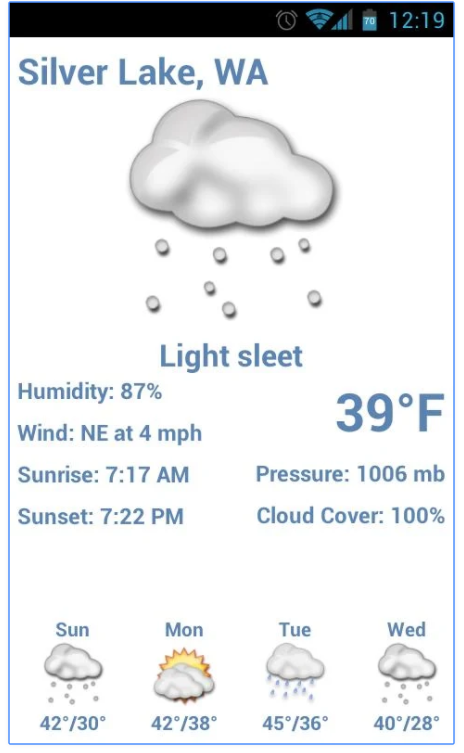
\includegraphics[width=6cm]{pesca4.png}

\caption{Datos sobre la meteorología}
\label{fig:pesca4}
\end{minipage}
\end{figure}
        \cleardoublepage



\chapter{Tecnología}
        \label{tec}
        
Una buena elección de la tecnología será una condición necesaria, aunque no suficiente, para llevar a cabo un proyecto con éxito.

En este capítulo presentamos las tecnologías utilizadas en el desarrollo de este proyecto. 
\section{Android SDK}
Android  \cite{2}  \cite{3} es un sistema operativo especialmente diseñado para dispositivos móviles. Permite el desarrollo de sus aplicaciones en un lenguaje similar al Java. El sistema operativo nos proporciona de manera sencilla todas las inferfaces para el desarrollo de las aplicaciones que puedan acceder a las funciones del teléfono.\\

\textbf{Android SDK}\\

El SDK de Android ofrece un conjunto de herramientas para el desarrollo de aplicaciones incluyendo:
\begin{itemize}
\item \textbf{Depurador de código}
\item \textbf{Simulador de dispositivos de la plataforma. basado en QEMU}. Siendo QEMU  un emulador de procesadores. 
\item\textbf{ Bibliotecas.}
\item \textbf{Documentación.}
\item \textbf{Ejemplos de código.}

\end{itemize}


\section{Eclipse }


Eclipse es un IDE en Java para
( ver Figura~\ref{fig:eclipse}) para el desarrollo de software. Fue creado por IBM como sucesor de una de sus herramientas y ahora está en manos de la Fundación Eclipse que es quien se encarga de seguir desarrollándolo.
Se decidió usar esta herramienta de desarrollo ya que es totalmente gratuita por lo que no encarece el precio del proyecto y porque el entorno que usamos en Android esta basado en este.  
\begin{figure}[H]
		\centering
		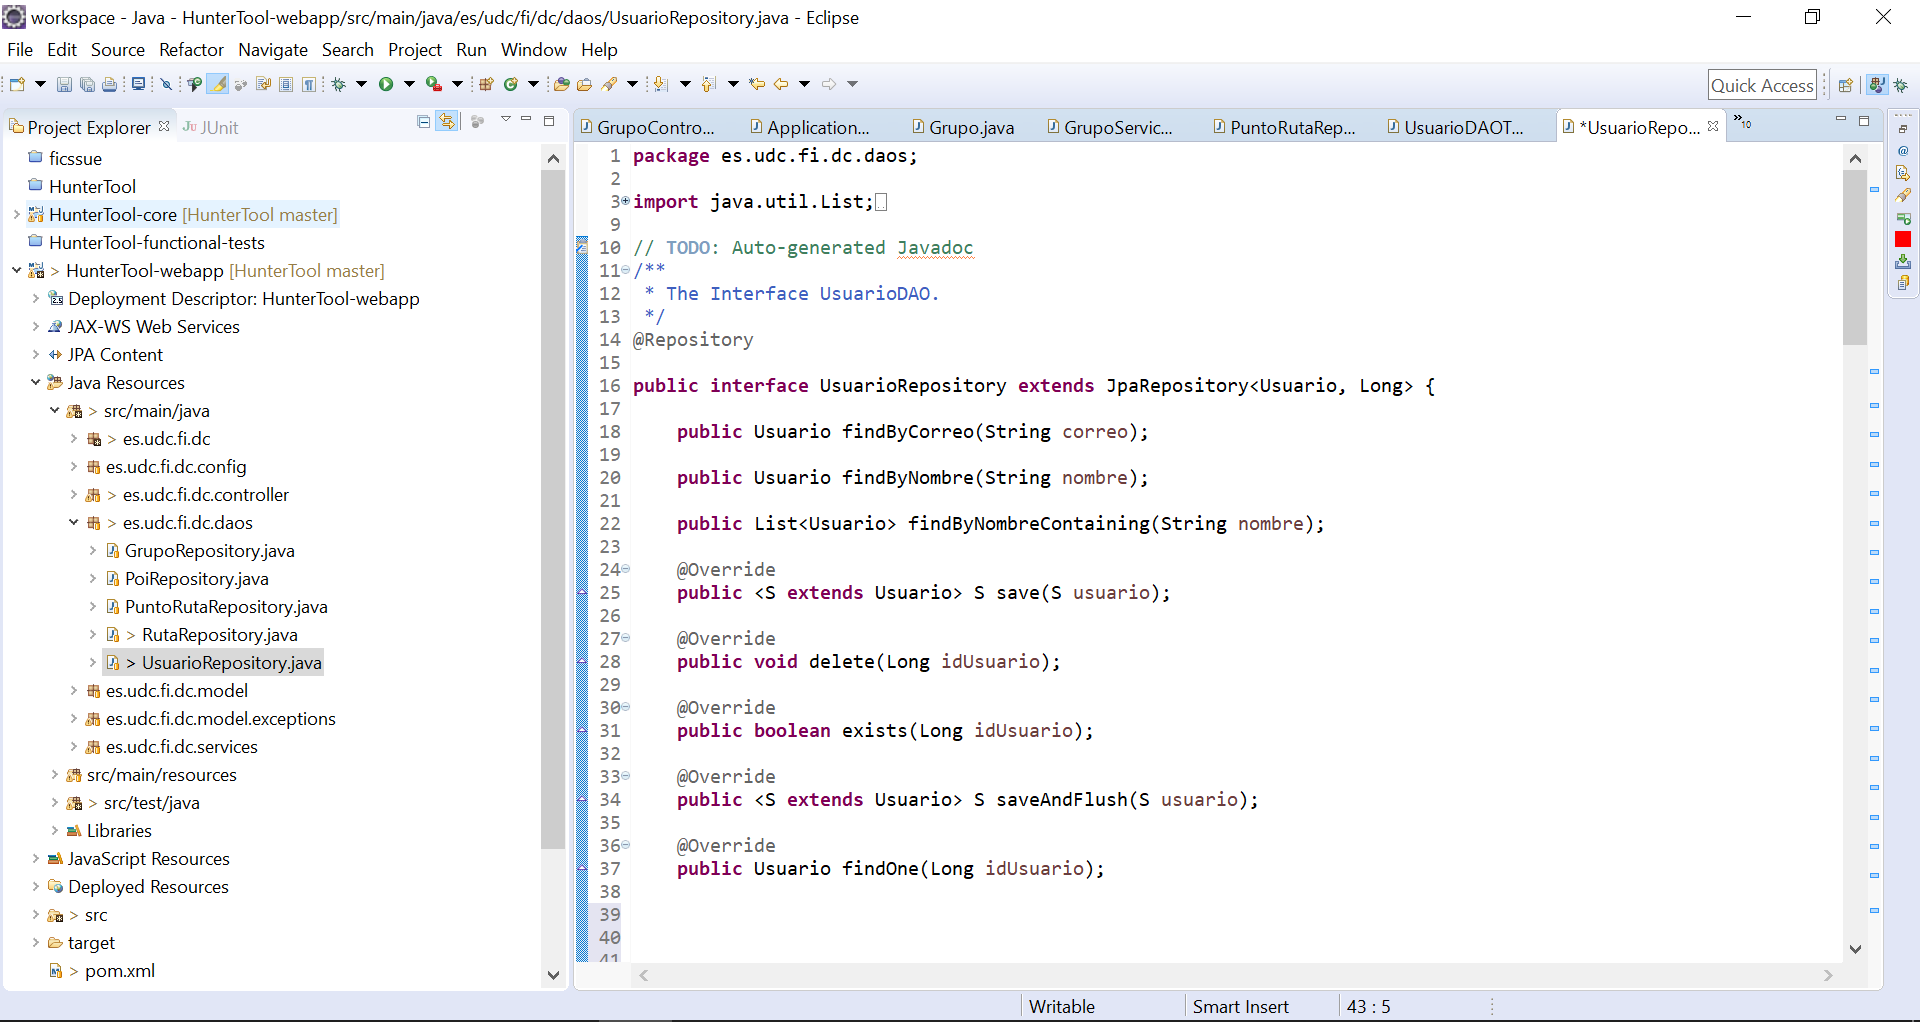
\includegraphics[width=\textwidth] {eclipse.png}
		\caption{Entorno de trabajo Eclipse }
		\label{fig:eclipse}
	\end{figure}
	
	
	
\section{Spring}
Spring es un framework de código abierto que tiene como objetivo ayudar al desarrollador a trabajar con otras APIs de manera más sencilla. Nos proporciona un modelo de programación y configuración integral para aplicaciones empresariales basadas en Java, en cualquier tipo de plataforma de implementación. 
	
Las funcionalidades principales que ofrece y por ello elegí, serían:

\begin{itemize}
\item \textbf{Programación orientada aspectos},paradigma que nos ayuda a eliminar dependencias entre módulos acortando las líneas de código de los servicios para así poder centrarnos en la lógica de la aplicación. Lo que conlleva reducir  la probabilidad de errores en la codificación o ineficiencias.


\item\textbf{ Inyección de dependencias}, patrón que ayuda a reducir el acoplamiento entre los distintos componentes de la aplicación. Esto lo consigue haciendo que una clase le proporcione a otra sus dependencias haciendo que la otra no tenga que crearlas ella misma. De este modo a través de un interfaz una clase tienes las dependencias de otra sin tener que preocuparse de la implementación de las mismas, lo que es favorable para reducir el acoplamiento.





\begin{lstlisting}[language=java,
 ,backgroundcolor=\color{backcolour},   
    commentstyle=\color{codegreen},
    keywordstyle=\color{magenta},
    numberstyle=\tiny\color{codegray},
    stringstyle=\color{codepurple}]  
@Service
public class GrupoServiceImpl implements GrupoService {

	@Autowired
	GrupoRepository grupoDAO;

	public void setGrupoDAO(GrupoRepository grupoDAO) {
		this.grupoDAO = grupoDAO;
	}


\end{lstlisting} 



\end{itemize}


\section{Android Studio}
Android Studio es el entorno de desarrollo integrado (IDE)  oficial para Android que nos ofrece las herramientas más rápidas para crear apps en todas las clases de dispositivos Android.
Además de ser una potente herramienta para la creación de código permite:

\begin{itemize}
\item Realizar compilaciones  de nuestro código para comprobar el estado de nuestras variables en los puntos que nosotros le indiquemos sin necesidad de general un APK.
\begin{figure}
		\centering
		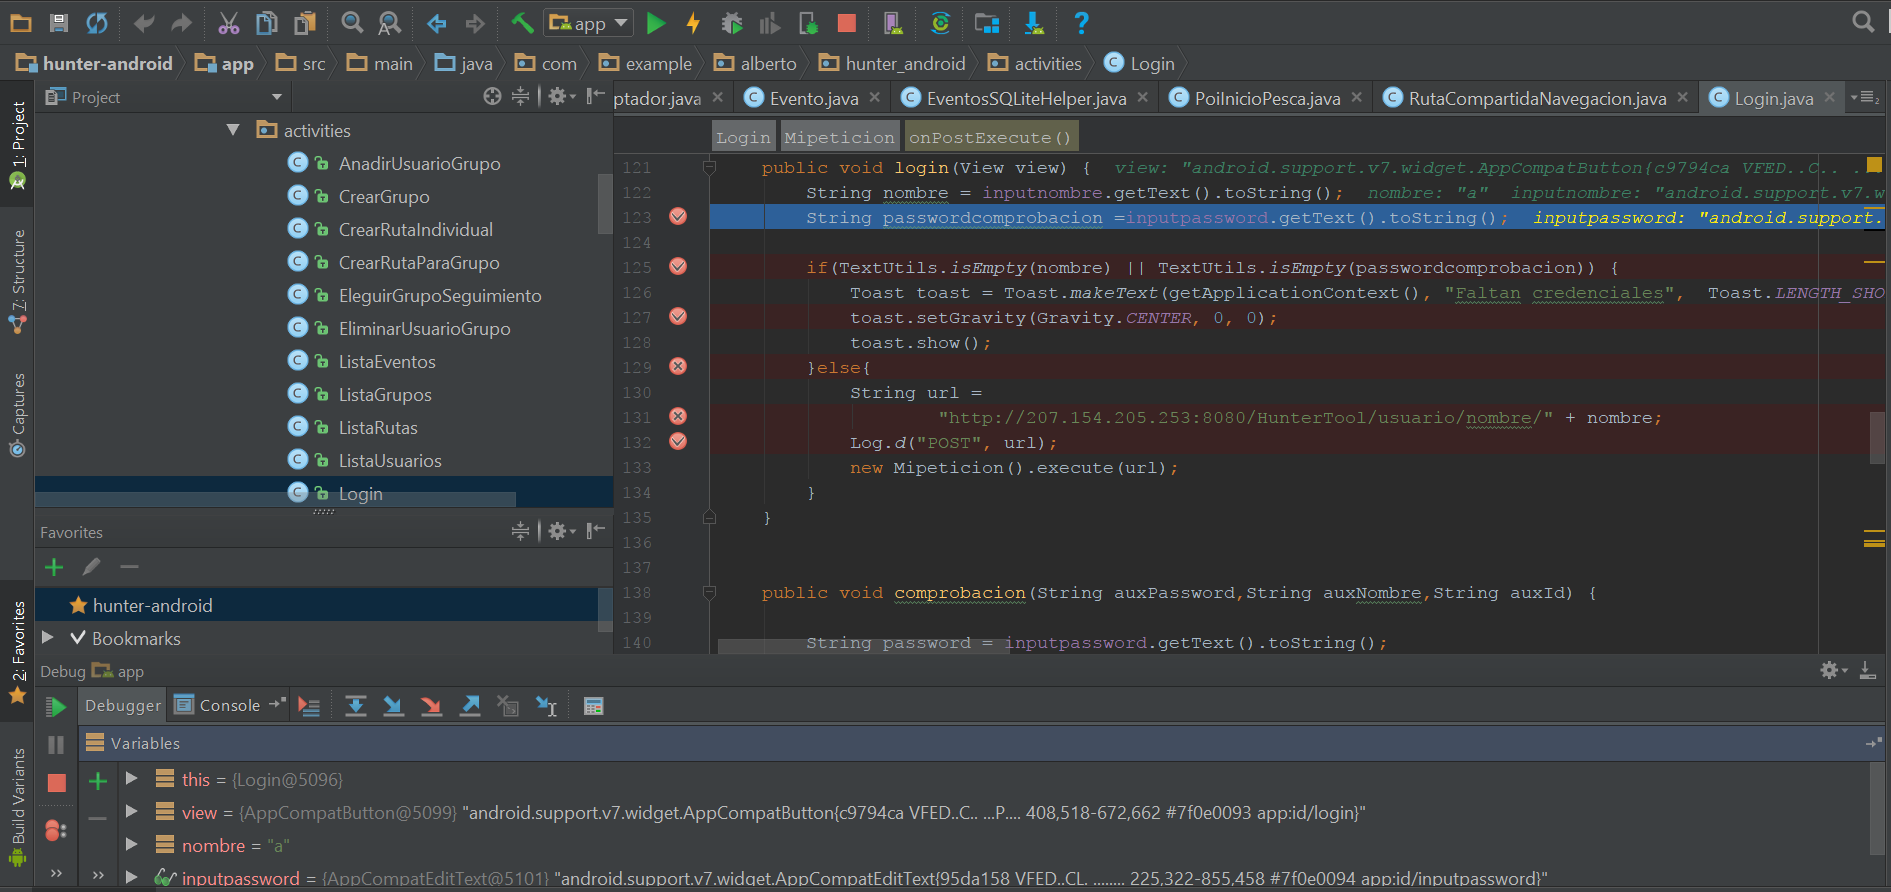
\includegraphics[width=\textwidth] {debug.png}
		\caption{Captura de pantalla realizando app debug }\label{fig:debug}
	\end{figure}

\item Generar un APK (Android Application Package) para la ejecución de nuestra aplicación móvil tanto de forma simulada, ayudándonos del simulador que nos proporciona o usando un móvil.
\end{itemize}
\begin{figure}
		\centering
		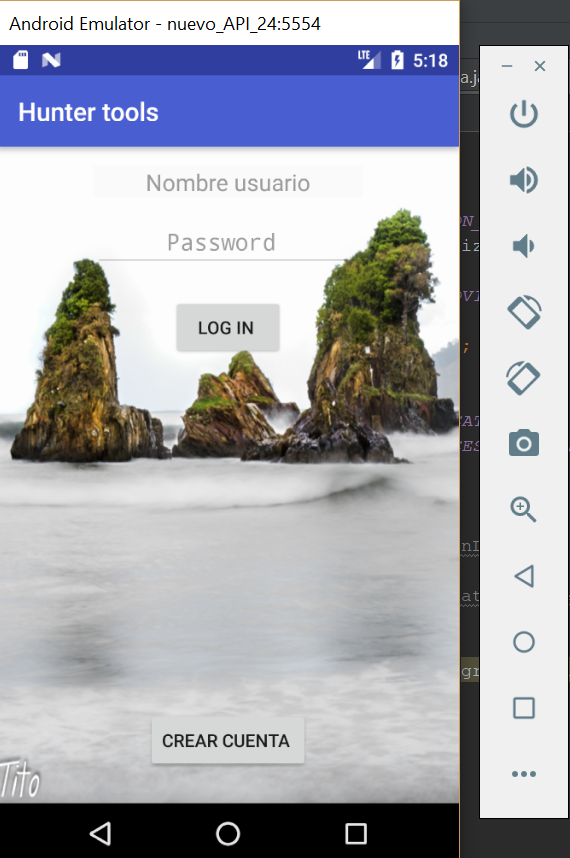
\includegraphics[width=0.6\textwidth] {emulador.png}
		\caption{Emulador de Android con mi aplicación}
		\label{fig:emulador}
	\end{figure}
 



\section{Git}
Git es un software para ayudarnos con el control de versiones  pensado para el mantenimiento de múltiples versiones de aplicaciones cuando estas tienen un número muy alto de archivos y queremos poder volver a un punto anterior o como copias de seguridad. A su vez, Git ofrece dos opciones para el control de versiones, una mediante un interfaz y otra mediante línea de comandos. Se escogió esta opción por las facilidades de uso que ofrece a la hora de realizar lo commits y el fácil nombrado de los mismos cuando queremos actualizar el repositorio.
\section{Maven}
Maven es una herramienta de software para la gestión y construcción de proyectos Java.
 Maven utiliza un Project Object Model (POM) en formato
XML para describir sus dependencias con otros módulos como jpa, firebase o postgrest. Viene con objetivos predefinidos para la compilación del código o su empaquetado. Se escogió por la buena estructuración de los paquetes que genera y por las similitudes que presenta frente al Gradle que usaremos en el entorno de desarrollo Android Studio.




\section{Gradle}
Gradle es una herramienta de software para la gestión, construcción de proyectos Android y gestor de dependencias. Ofrece
  herramientas de compilación avanzadas, para automatizar y administrar el proceso de compilación, y al mismo tiempo te permite definir configuraciones de compilación personalizadas.



\section{Jackson}

Jackson es un parseador para el desarrollo de Servicios Web en java. Implementa un conjunto de   herramientas de procesamiento de datos para Java haciendo que el desarrollo de servicios Rest sean más simples. Se eligió esta opción por lo sencillo que hacia el mapeo de objetos en las peticiones a JSON y dado que se usa el framework Spring este parseador ya viene integrado.








\section{JPA/Hibernate}
Hibernate es una herramienta de mapeo objeto-relacional para la plataforma Java que ayuda a la transformación de objetos del modelo a una entidad de la base de datos persistente. Este mapeo ayuda a  no tener que definir la entidad directamente en nuestro gestor de base de datos. Para conseguir esto debemos usar las anotaciones pertinentes en el entorno de desarrollo (Eclipse) sin necesidad de acceder al gestor de base de datos en ningún momento. Una vez puestas las anotaciones los accesos a datos de la  bases de datos pasan a ser muy sencillos.





\section{PostgreSQL}
PostgreSQL es un gestor de bases de datos objecto-relacional  que permite trabajar con grandes cargas de datos consiguiendo una tolerancia alta a errores.
Se decidió usar este gestor porque tiene una gran adaptabilidad a otros entornos de trabajo lo que ayuda a ganar agilidad y eficiencia. También nos proporciona  el PgAdmin que facilita la gestión y administración de bases de datos ya sea mediante instrucciones SQL o con ayuda de un entorno gráfico. Permite acceder a todas las funcionalidades de la base de datos, consulta, manipulación y gestión de datos.
\section{JUnit}
JUnit es el framework de testing para Java más extendido.
Permite la ejecución de clases Java para evaluar el comportamiento de los métodos a testar.


\vspace{1cm}

Con estas tecnologías se ha llevado a cabo la construcción de los distintos componentes del sistema siguiendo los pasos que comentaremos en el próximo capítulo.

        \cleardoublepage

\chapter{Proceso de ingeniería}
		En este capítulo se justifica la elección y se describe la metodología de desarrollo sobre la que se apoya el proceso de ingeniería. En este proyecto se ha empleado una metodología ágil, Scrum. 



\section{Scrum}

El Scrum es una  Metodología ágil \cite{6} \cite{9} que se usa para estructurar y gestionar proyectos, y para minimizar los riesgos durante la realización del mismo.
Esta metodología esta basada en ciclos iterativos cortos e incrementales, lo que se traduce en una gran flexibilidad a la hora de adaptarse a cambios que surjan duran el desarrollo del proyecto.
Entre las ventajas de Scrum se encuentran la baja carga de burocracia y documentación, productividad, calidad y que se realiza un seguimiento diario de los avances del proyecto, logrando una comunicación activa y constante en el equipo de trabajo.\\
A continuación se describen los principales  de la metodoligía Scrum.


\subsection{Historias de usuario}
Las historias de usuario son los requisitos vistos desde el punto de vista del cliente, es decir, acciones que el usuario llevará a cabo durante el uso del la aplicación. Son la unidad básica detrabajo y se caracteriza por ser:
\begin{itemize}
\item Independientes
 \item Negociables
  \item Estimables
  \item Pequeñas
   \item Tangibles
    
\end{itemize}

Las historias en este proyecto serán las siguientes:


\begin{itemize}
\item Diseño capa intermedia
\item Implementación del servicio Rest
\item Iniciar sesión  
 \item Gestión de puntos de interés (PDI)
  \item Gestión de grupos
  \item Iniciar una ruta individual
   \item Iniciar la ruta compartida
   \item Realización de la memoria.
    
\end{itemize}
 Estas historias anteriormente citadas serán divididas en cada Sprint en pequeñas tareas mas fáciles de manejar. Una tarea es la acción que debe implementar el desarrollador para que se pueda ejecutar parte de la historia, esta está en un lenguaje técnico. Estas tareas reflejan en la mayoría de los casos los denominados casos de uso que comentaremos posteriormente.

\subsection{Sprint}

Por Sprint entendemos un bloque de tiempo fijo, normalmente de 3 o 4 semanas en el que
se crea una versión de nuestra aplicación que se irá incrementando de tamaño
según van avanzando los Sprints. Los Sprints se pueden considerar como pequeños
proyectos ya que al final de cada uno de ellos debemos tener un producto
operativo, es decir, que responda a la historia o historias de usuario planteadas en él.



\subsection{Participantes}
\begin{itemize}
\item \textbf{Product Owner}\\
Es el responsable del producto, de priorizar los user stories y de decidir si el sistema las cumple. En general , es un representante del cliente u otro stakeholder


\item \textbf{Scrum Master}\\
Es el encargado de liderar la reuniones y ayudar al equipo en los problemas que tengan  en la implementación de la metodología. Debe minimizar las imposibilidades que surgen en el desarrollo del proyecto para que se cumplan los objetivos. Además debe promover la comunicación entre los integrantes del grupo para generar la motivación necesaria para conseguir los objetivos en plazo.




\item  \textbf{Scrum Team}\\
Son los encargados de desarrollar y llevar acabo las tareas de los sprints. En si son quienes realizan las tareas que finalmente generan el producto que se va a entregar.


\item  \textbf{Cliente}\\
Recibe el producto y puede influir en el proceso, entregando sus ideas o comentarios respecto al desarrollo a través del feedback con el product owner y el equipo sobre las versiones del producto. 
\end{itemize}

\subsection{Cómo funciona el Proceso}



\begin{figure}
		\centering
		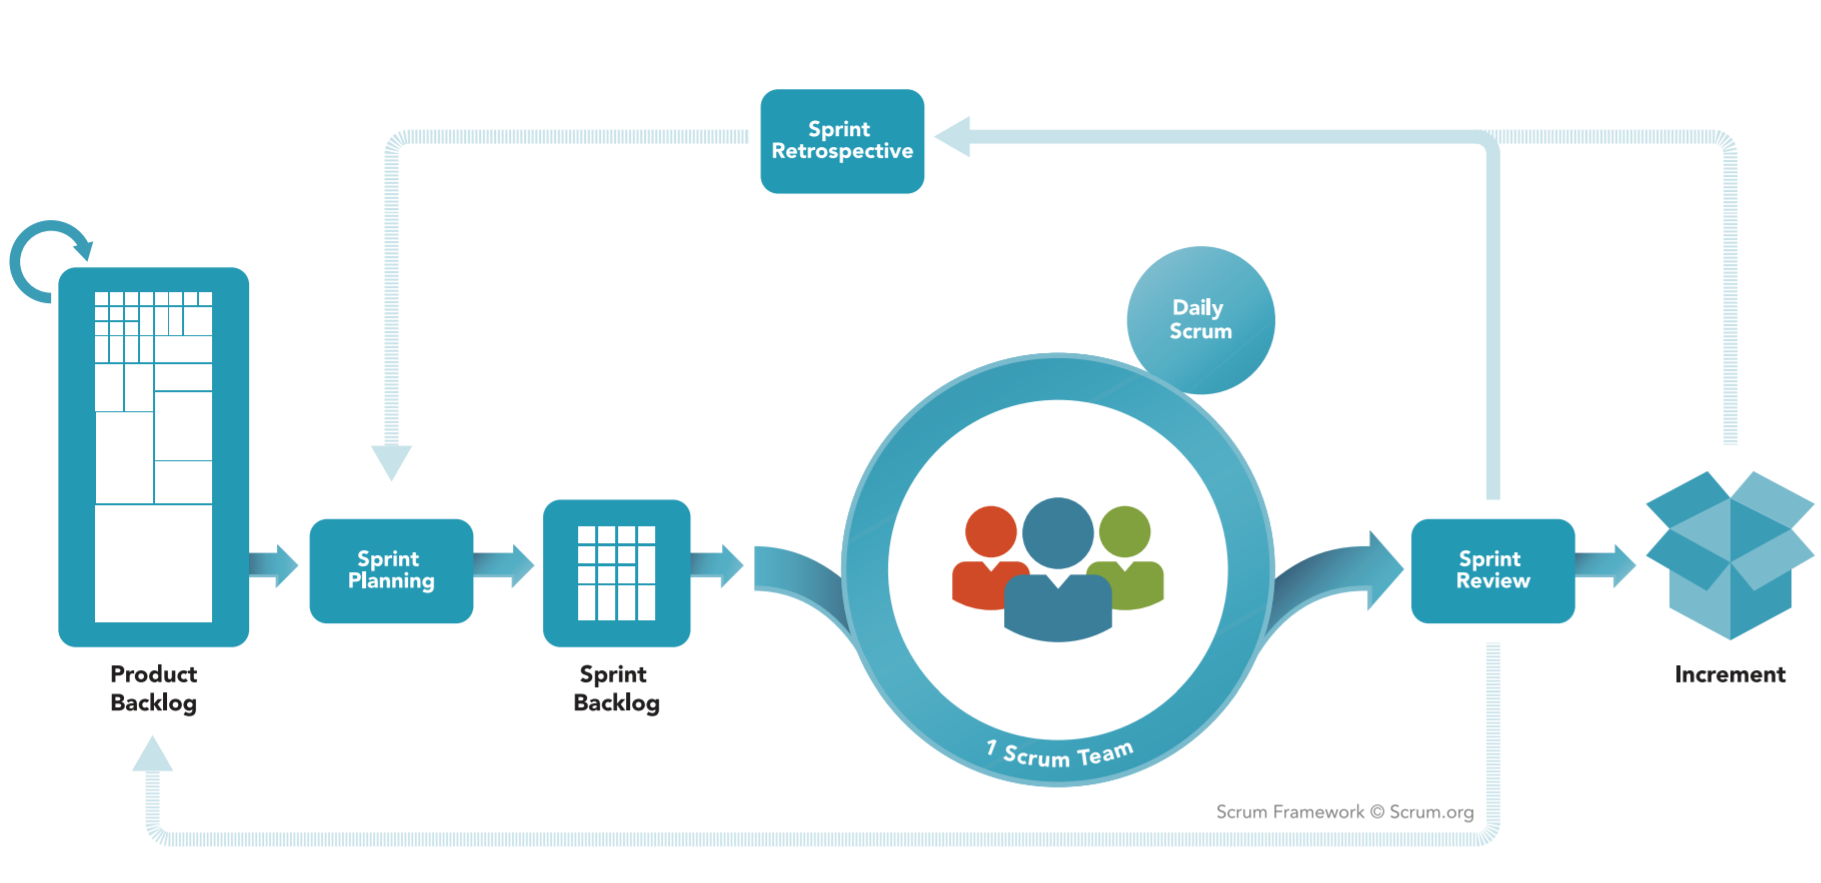
\includegraphics[width=\textwidth] {scrum.jpg}
		\caption{Metodología Scrum }
		\label{fig:scrum}
	\end{figure} 


El proceso comienza con la definición del Product Backlog. De este Product Backlog  se irán obteniendo las historias para los distintos sprints. El proceso general se puede ver en la figura~\ref{fig:scrum}. A continuacion comentaremos sus partes:
\begin{itemize}
\item \textbf{Definición del Product Backlog}. Figura~\ref{fig:product}
Es una lista con las funcionalidad de la aplicación.
Estas funcionalidades que se definen en el Product Owner son las historias del usuario, es decir, es lo que el usuario quiere hacer en la aplicación y por tanto en muchos casos cada historia puede contener varios casos de uso. \\
Está elaborado por el Product Owner y las funcionalidad están ordenadas de mayor a menor importancia para el cliente. La finalidad del Product Owner es plantear lo que hay que hacer.
Con las historias ordenadas se indicarán los Sprints que serán necesarios pudiendo hacer  varias historias en un mismo Sprint pero nunca una historia dividida en dos Sprints. 

 
 \begin{figure}
		\centering
		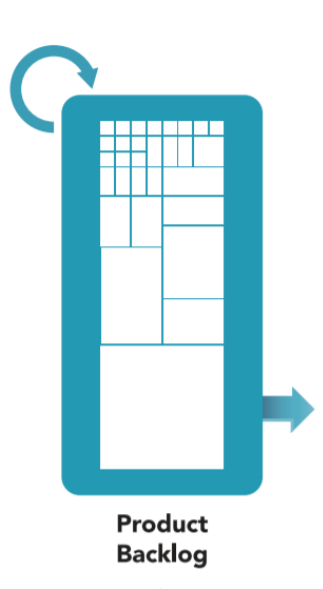
\includegraphics[width=0.2\textwidth] {product.png}
		\caption{Parte metodología Scrum, Product Backlog }\label{fig:product}
	\end{figure} 


\item \textbf{Sprint Planning Meeting}. Figura~\ref{fig:planing}\\
 Esta reunión se hace al comienzo de cada Sprint y se define cómo se va a enfocar el proyecto, se revisan las historias con mayor prioridad y se decide el Sprint backlog.
\begin{figure}[H]
		\centering
		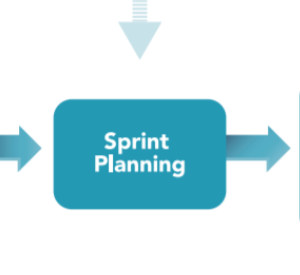
\includegraphics[width=0.3\textwidth] {planing.png}
		\caption{Parte metodología Scrum, Sprint Planning }\label{fig:planing}
	\end{figure} 

\item \textbf{Sprint Backlog}. figura~\ref{fig:sprint}\\
Es el conjunto de historias del Product Backlog que se decidirán hacer en el Sprint, estando ordenadas de mayor a menor prioridad. Una vez completado los miembros del equipo dividirán las historias en tareas más pequeñas y más manejables, si es necesario.

\begin{figure}[H]
		\centering
		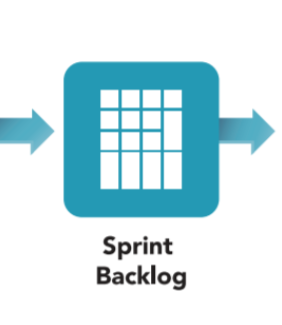
\includegraphics[width=0.3\textwidth] {sprint.png}
		\caption{Parte metodología Scrum, Sprint Backlog }\label{fig:sprint}
	\end{figure} 

 
 
\item \textbf{Daily Scrum o Stand-up Meeting. Figura~\ref{fig:daily}}\\
Es una reunión breve que se realiza cada mañana mientras dura el periodo de Sprint. 
En estas reuniones si algún miembro del equipo encuentra algún problema  se comenta y se trata de buscar la solución. El scrum master es el encargado de lidiar con los inconvenientes encontrados.

\begin{figure}[H]
		\centering
		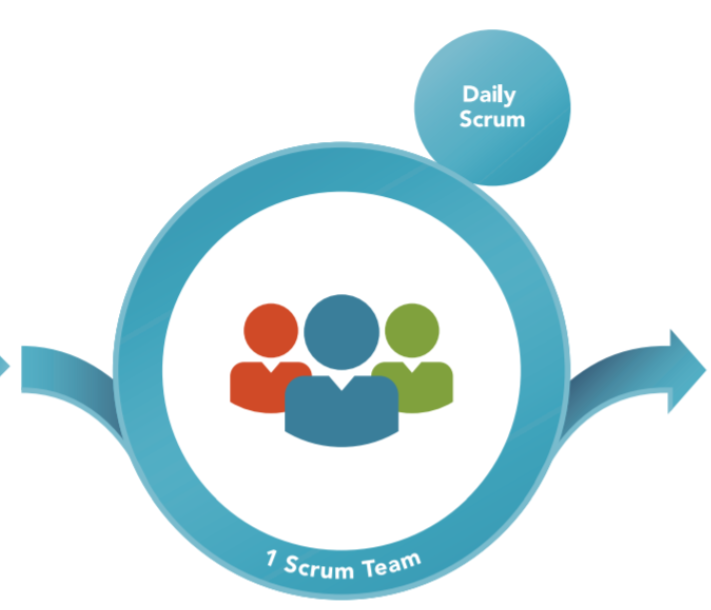
\includegraphics[width=0.3\textwidth] {daily.png}
		\caption{Parte metodología Scrum, Daily Scrum }\label{fig:daily}
	\end{figure} 

\item\textbf{ Sprint Review}\\
Esta sería la primera reunión una vez acabado el Sprint. En ella se deberían plantear las tareas acabadas y se debería ver un avance claro para ser presentado al cliente. Las tareas inacabas las deberían ser devueltas al Product Backlog y si hiciera falta volver a calcular las prioridades.

 \item \textbf{Sprint Retrospective}\\
  El equipo revisa los objetivos cumplidos del Sprint terminado. Se anota lo bueno y lo malo, para no volver a repetir los errores. Esta etapa se centra en el cómo se realiza el proyecto para si hay algún error en el desarrollo poder resolverlo en el siguiente Sprint.
\end{itemize}



\section{Adaptación la metodología a este proyecto }
 Debido a la naturaleza de un Trabajo de fin de grado  debimos realizar una serie de cambios o adaptaciones en ciertos elementos como fueron los siguientes :
\subsection{Participantes}
Los participantes fueron los siguientes:
\begin{itemize}
\item El Product Owner interpretado por los  directores.
\item El cliente tambien fue desempeñado por los directores.
\item El Scrum Master no se usó puesto que se decidió 
 user scrum program.
\item  Y el equipo solo estuvo formado por el alumno.

\end{itemize}

\subsection{Sprints}
Cada sprint siempre tuvo una duración establecida de 4 semanas y 5 horas cada día aunque la carga de trabajo variaba en algún Sprint.


\subsection{Reuniones}

En el apartado de las reuniones siempre se establecían las tareas a realizar en cada jornada de trabajo. Al finalizar cada Sprint se realizaban reuniones con los directores y se aprovechaba para la planificación de la siguiente.\\

Una vez adaptada la metodología a este proyecto encontramos las siguientes ventajas a su uso:

\begin{itemize}
\item Ayuda a estar más centrado en el producto durante el desarrollo del proyecto ya que no existe la preocupación por establecer las siguientes tareas.  Estas ya quedaron indicadas en el sprint. 



\item En ocasiones al ir avanzando en el desarrollo aparecen nuevas funcionalidades que se pueden ir añadiendo al Product Backlog. Esto lo podemos hacer siempre y cuando nos ciñamos al Sprint Backlog
 para saber la tarea que realizar en ese momento.


\item  Las historias de usuario se irán dividiendo en tareas que se puedan realizar durante el sprint. De este modo una vez acabado el sprint tengamos un producto potencialmente entregable.\\

Dado el poco conocimiento de la metodología Scrum antes de la realización del proyecto, el ir avanzando en el proceso ayuda a adquirir conocimientos. Los cuales ayudarán a estimar mejor la duración e importancia de los elementos que se añaden al Sprint Backlog.


\item
Durante el desarrollo del proyecto hay ciertas funcionalidades que pueden cambiar. Empleando los principios de las metodologías ágiles en cada iteración haremos que el proyecto sea mas adaptable antes nuevos requisitos y cambios.

\end{itemize}

		\cleardoublepage

\chapter{Analisis}
		
  
  
\section{Análisis de Requisitos}


En esta aplicación móvil para actividades a campo abierto objetivo de este proyecto, se establecieron una seria de requisitos generales que debería cumplir la aplicación.\\

El registro del usuario para poder comenzar a usarla.\\

La creación de puntos de interés marcados en un mapa con nombre, descripción y un punto en el mapa con o sin señal GPS clasificados en tipo, caza o pesca. \\

Se podrán guardar las rutas seguidas por un usuario en sus caminatas por cualquier tipo de terrero.\\

El usuario también podrá crear grupos con los usuarios que quiera y los integrantes del mismo poder añadir a otros, el resultado de esta funcionalidad es la que permitirá posteriormente  crear rutas conjuntas. Para crear una ruta conjunta primero se elige el grupo del que se hará el seguimiento y se enviarán  las invitaciones para participar en él a cada integrante del grupo. Estas invitaciones en el caso de ser aceptadas llevaran al usuario a un mapa y periódicamente se irán realizando actualizaciones de las posiciones del resto de integrantes del grupo anteriormente indicado. Finalmente se podrán ver las rutas conjuntas igual que las individuales.
\subsection{Actores}

Los únicos actores que se presentan en la  aplicación son los siguientes:
\begin{itemize}
\item \textbf{Usuario no  autenticado}.Usuario que no está autenticado en la aplicación y que
se le permite registrarse en el  sistema o iniciar sesión si la ya se registro en otro momento.
\item \textbf{Usuario  autenticado}.Usuario autenticado que puede acceder a todas as funcionalidades
del sistema.
\end{itemize}
\subsection{Casos de uso}
A continuación, en esta sección, se exponen los requisitos funcionales que surgen de los requisitos generales planteados en el punto anterior.
\subsubsection{• Usuario no autenticado}
\begin{itemize}
\item\textbf{ \textit{R1}  Registrarse en la aplicación.}
 El usuario podrá darse de alta en el sistema
introduciendo sus datos en el formulario que se le indican. Una vez registrado se iniciará sesión
automáticamente con el nuevo perfil.

\item \textbf{\textit{R2} Iniciar sesión en la aplicación. }
El usuario ya registrado podrá, con
sus credenciales, autenticarse en el  sistema. Se pedirá o nombre del usuario la aplicación y  su contraseña. Se guardará el estado en el terminal hasta que el usuario decida desconectarse.
\end{itemize} 
\begin{figure}[H]
		\centering
		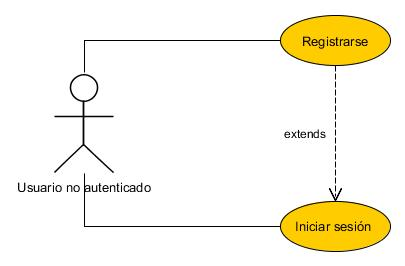
\includegraphics[width=0.75\textwidth] {usuario-no-autenticado.jpg}
		\caption{Casos de uso del actor Usuario No Autenticado }
	\end{figure}
\subsubsection{• Usuario  autenticado}
Para hacer un poco más comprensible dividiré los casos de uso del usuario autenticado por grupos funcionales.
\begin{itemize}
\item \textbf{Gestión de puntos de interés}\\
Aquí se describirán  los casos de uso relacionados con la gestión  de la  información del  los puntos de interés
\begin{itemize}
\item\textbf{\textit{ R-PDI-1 Guardar Punto De Interés caza}}, el usuario podrá guardar un punto concreto, de caza, asociado a un par de coordenadas pudiendo añadirle un nombre y una descripción.
\item\textit{ \textbf{R-PDI-2 Guardar Punto De Interés pesca}}, el caso de uno es similar al de anterior pero este es para el tipo de pesca.
\item \textbf{\textit{R-PDI-3 Eliminar PDI}}, el usuario podrá seleccionar un punto o una lista de puntos para ser borrados.
\item \textbf{\textit{R-PDI-4 Buscar los PDI}}, permite ver todos los puntos de interés de cada tipo por separado pintados en un mapa y pudiendo ciclar en ellos para conocer su nombre y descripción.
\end{itemize} 

\begin{figure}[H]
		\centering
		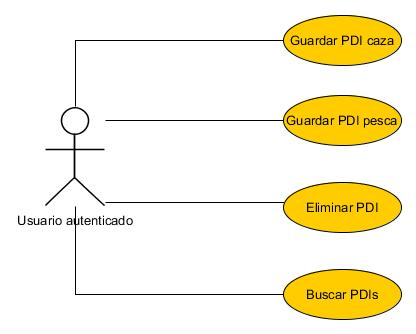
\includegraphics[width=0.75\textwidth] {PDI.jpg}
		\caption{Casos de uso de gestión de puntos de interés }
	\end{figure}
\item \textbf{Gestión de grupos}
\begin{itemize}
\item\textbf{ \textit{R-G-1 Crear grupo}}, el usuario crea un grupo con nombre único.
\item\textbf{\textit{ R-G-2 Añadir integrantes}}, el usuario busca en la base de datos los usuarios que quiere integrar en el grupo previamente creado.
\item \textbf{\textit{R-G-3 Eliminar integrantes}}, el usuario puede eliminar los integrantes que vea pertinentes.
\item \textbf{\textit{R-G-4 Ver grupos}}, el sistema listarla los grupos en los que el usuario está registrado.
\item \textbf{\textit{R-G-5 Ver integrantes grupo}}, el sistema permitirá ver los integrantes del grupo que el usuario indique , previo listado del caso de uso R-G-4. 

\end{itemize} 

\begin{figure}[H]
		\centering
		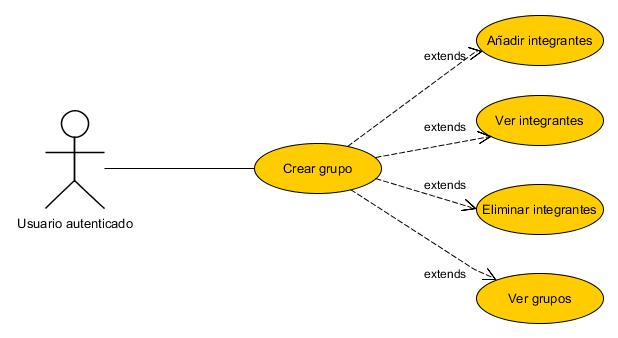
\includegraphics[width=0.75\textwidth] {grupo.jpg}
		\caption{Casos de uso de gestión de grupos de usuarios }
	\end{figure}
\item \textbf{Gestión de rutas,}el usuario iniciará una navegación privada siendo guardada la ruta seguida.
\begin{itemize}
\item \textbf\textit{{R-R-1 Crear ruta privada}}, el usuario registra la ruta con un nombre.
\begin{itemize}
\item \textbf{\textit{R-R-1.1}} Iniciar ruta, el sistema comienza a guardar las coordenadas por la que el usuario esta navegando y dibujando la ruta en el mapa. Las coordenadas se irán guardando periódicamente.
\item\textbf{ \textit{R-R-1.2}} Parar ruta, permite parar la navegación, tanto de guardar las coordenadas como de pintar la ruta seguida.
\item \textbf{\textit{R-R-1.3}} Guardar ruta, el sistema guarda los últimos puntos que quedaban sin actualizar y ejecuta el caso de uso ver ruta en el mapa(R-R-4).
\end{itemize}

\item \textbf{\textit{R-R-2 Crear ruta compartida}}, este caso de uso permite guardar la ruta seguida por el usuario y al mismo tiempo ver la posición del resto de integrantes de un grupo, anteriormente seleccionado, en tiempo real. Este caso de uso también enviaría a los integrantes del grupo una invitación a dicha ruta.
\begin{itemize}
\item \textbf{\textit{R-R-2.1 Iniciar ruta}}, se comienza a guardar y dibujar la ruta en el mapa. Por otra parte se comienza el seguimiento del resto de usuario que estén también navegando. Como también una actualización parcial de la ruta seguida en el servidor.
\item \textbf{\textit{R-R-2.2 Parar ruta}}, se para la navegación y se deja de actualizar la posición al resto de usuario de la ruta compartida.
\item \textbf{\textit{R-R-2.3 Finalizar ruta}}, se guardan los puntos que faltan de enviar al servidor y se deja de enviar datos al resto de integrantes.
\end{itemize}
\item \textbf{\textit{R-R-3 Listar rutas} }, permite al usuario ver todas las rutas realizadas tanto de manera privada como de manera compartida.
\item \textbf{\textit{R-R-4 Ver ruta en mapa}}, el sistema dibuja en un mapa la ruta seguida y previamente seleccionada.
\item \textbf{\textit{R-R-5 Eliminar ruta}}, permite al usuario borrar de la aplicación la ruta indicada.

\end{itemize} 
\end{itemize}
\begin{figure}[H]
		\centering
		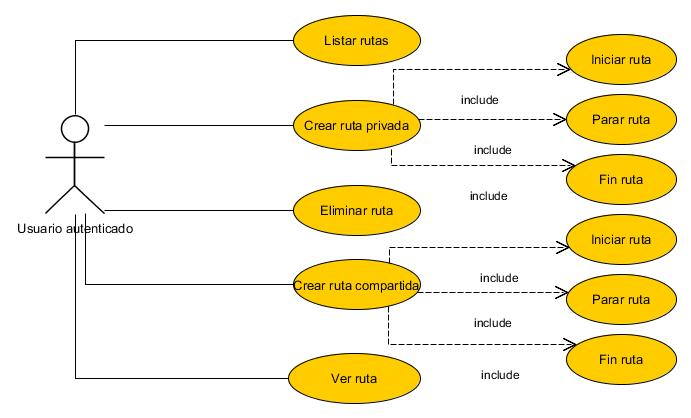
\includegraphics[width=0.75\textwidth] {rutas.jpg}
		\caption{Casos de uso de gestión de rutas }
	\end{figure}

\newpage
\section{Maquetas}
Comenzamos creando las maquetas de como debería que ser a interface del usuario.
Se busca que sea una interface simple y intuitiva.
Para esto, se intentarán seguir las pautas y usar lo  máximo posible los elementos de Material
Design [6].
Material Design es un lenguaje de diseñoo para distintas plataformas y dispositivos,
creada por el diseñador graco de Google Matas Duarte. Ofrece una guía  para ofrecer
a los usuarios una experiencia común y habitual entre distintas aplicaciones.


	
	
	
	\begin{figure}[htbp]
\begin{minipage}[b]{0.5\linewidth} %Una minipágina que cubre la mitad de la página
\centering
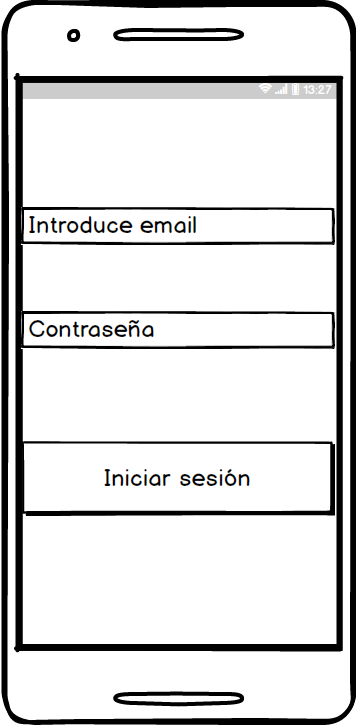
\includegraphics[width=6cm]{maqueta/Iniciar.png}
 \label{figura1}
\caption{Inisiar sesión}

\end{minipage}
\hspace{0.5cm} % Si queremos tener un poco de espacio entre las dos figuras
\begin{minipage}[b]{0.5\linewidth}
\centering
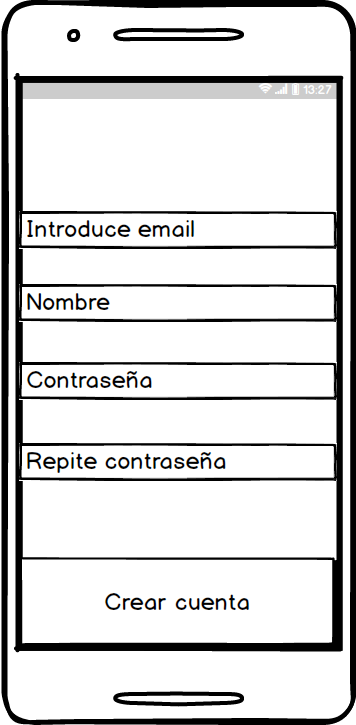
\includegraphics[width=6cm]{maqueta/Registrarse.png}
 \label{figura2}
\caption{Registrar usuario}

\end{minipage}
\end{figure}










	
	\begin{figure}[htbp]
\begin{minipage}[b]{0.5\linewidth} %Una minipágina que cubre la mitad de la página
\centering
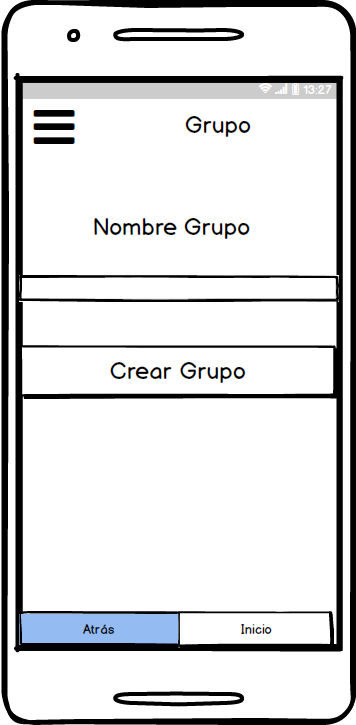
\includegraphics[width=6cm]{maqueta/Crear-Grupo.png}
 \label{figura1}
\caption{Crear grupo}

\end{minipage}
\hspace{0.5cm} % Si queremos tener un poco de espacio entre las dos figuras
\begin{minipage}[b]{0.5\linewidth}
\centering
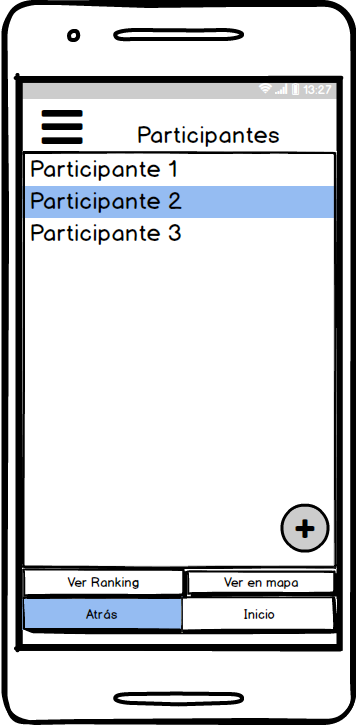
\includegraphics[width=6cm]{maqueta/Ver-Miembros-grupo.png}
 \label{figura2}
\caption{Añadir usuarios a grupo}

\end{minipage}
\end{figure}
	
	
	
	
	
	
	
	
	
	
	
	
	
	
	
	
	
	\begin{figure}[htbp]
\begin{minipage}[b]{0.5\linewidth} %Una minipágina que cubre la mitad de la página
\centering
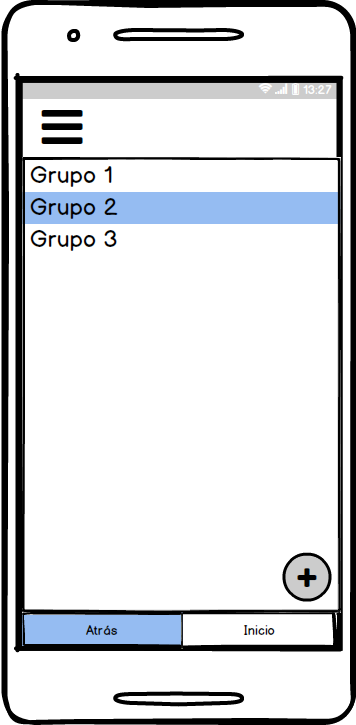
\includegraphics[width=6cm]{maqueta/lista-grupos.png}
 \label{figura1}
\caption{Listar grupos}

\end{minipage}
\hspace{0.5cm} % Si queremos tener un poco de espacio entre las dos figuras
\begin{minipage}[b]{0.5\linewidth}
\centering
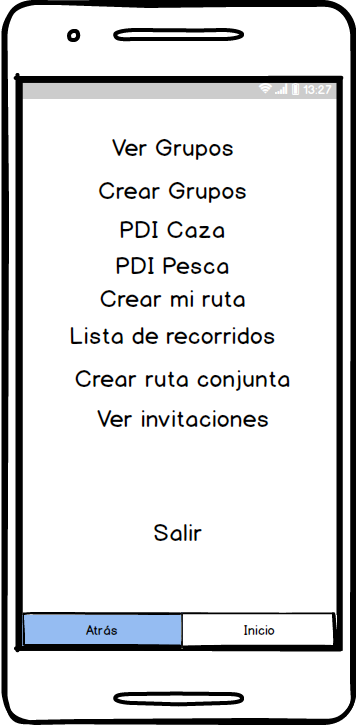
\includegraphics[width=6cm]{maqueta/opciones.png}
 \label{figura2}
\caption{Opciones generales}

\end{minipage}
\end{figure}
	















	\begin{figure}[htbp]
\begin{minipage}[b]{0.5\linewidth} %Una minipágina que cubre la mitad de la página
\centering
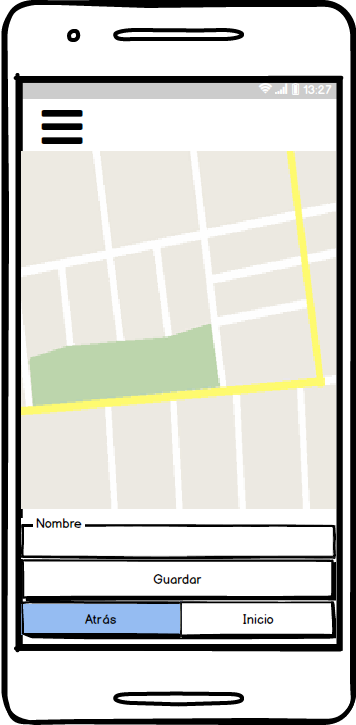
\includegraphics[width=6cm]{maqueta/pdi1.png}
 \label{figura1}
\caption{Crear PDI}

\end{minipage}
\hspace{0.5cm} % Si queremos tener un poco de espacio entre las dos figuras
\begin{minipage}[b]{0.5\linewidth}
\centering
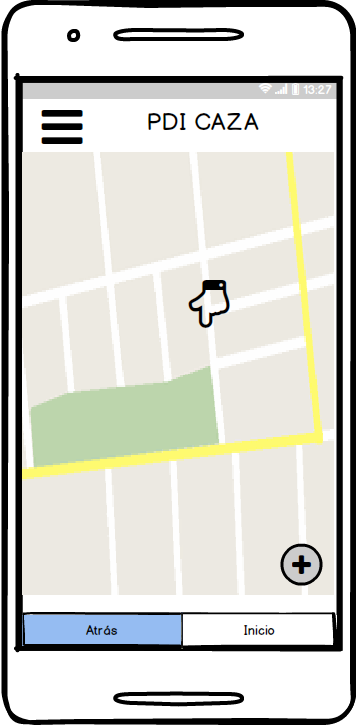
\includegraphics[width=6cm]{maqueta/pdi2.png}
 \label{figura2}
\caption{Visualizar PDIs}

\end{minipage}
\end{figure}
	

	\begin{figure}[htbp]
\begin{minipage}[b]{0.5\linewidth} %Una minipágina que cubre la mitad de la página
\centering
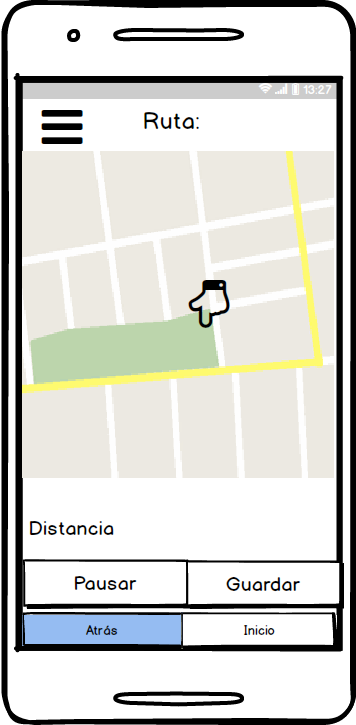
\includegraphics[width=6cm]{maqueta/Trayecto-actual.png}
 \label{figura1}
\caption{Ruta individual}

\end{minipage}
\hspace{0.5cm} % Si queremos tener un poco de espacio entre las dos figuras
\begin{minipage}[b]{0.5\linewidth}
\centering
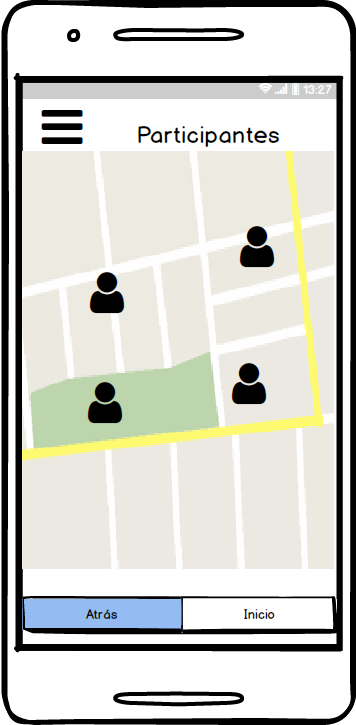
\includegraphics[width=6cm]{maqueta/Trayecto-actual-compartido.png}
 \label{figura2}
\caption{Ruta compartida}

\end{minipage}
\end{figure}



		\cleardoublepage


\chapter{Seguimento}


 En este capítulo se comentará el proceso seguido para la realización de este proyecto detallando la planificación, diseño y el desarrollo del mismo estructurado en etapas.
 
\section{Planificación}

Una vez hecho el análisis, conocidos los objetivos que se quieren alcanzar en este proyecto y las herramientas que se utilizarán  empezaremos con la planificación del mismo.

Un punto muy  importante a tener en cuenta a la hora de realizar una planificación sería conocer los recursos y el tiempo del que disponemos.




Éste punto tan crucial se acentúa ya que este proyecto será hecho por una única persona lo que producirá sobrecargas en la planificación. Esto normalmente no es así ya que los proyectos se realizan por grupos de trabajos y muchas tareas pueden realizarse en paralelo disminuyendo apreciablemente la duración del proyecto.

Para realizar la planificación del proyecto hemos dividido el proyecto en tareas con unos objetivos bien marcados(Product Backlog). A su vez al seguir la metodología Scrum dividimos el proyecto en etapas(Sprint) de tiempo donde incluimos las tareas a realizar.
En todas estas etapas incluimos los siguientes pasos:
 
 


\begin{itemize}
\item Definición del Sprint Backlog, documento que recoge las tareas a realizar y quién las desempeña. En esta caso al solo trabajar yo en el proyecto haré todas las tareas.


\item División del Sprint Backlog en tareas más sencillas y abordables(Backlog items). 



\item Diseño de cada una de las tareas del punto anterior.
\item  Implementacion de las tareas.
\item Pruebas.
\end{itemize}

\begin{figure}[H]
		\centering
		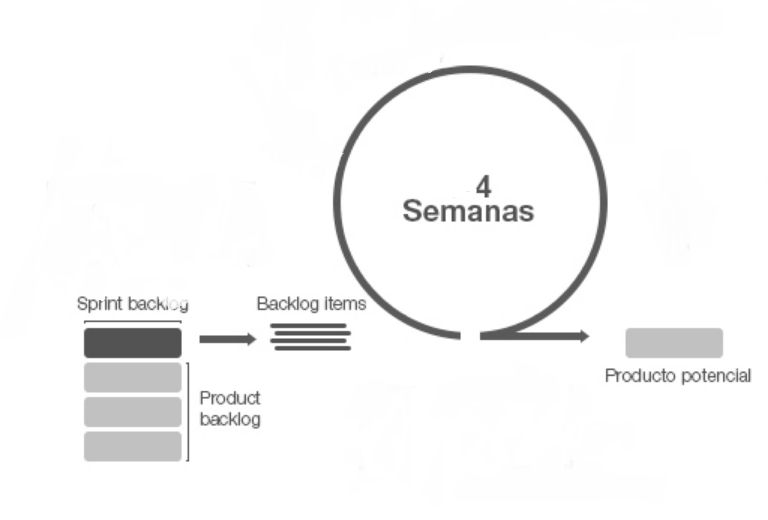
\includegraphics[width=0.75\textwidth] {backlog.png}
		\caption{Pasos metodología Scrum}
	\end{figure} 

\section{Estimación de tiempos y costes}
 A continuación en la tabla siguiente se ha realizado una estimación de tiempos y de costes de este proyecto.
 Cuando se realiza una estimación de costes tenemos que tener en cuenta los gastos en material, licencias y los gastos propios. En este caso los gastos de materias y de licencias en cero ya que el material usado era aportado por el alumno y las licencias eran todas gratuitas.
 En la siguiente tabla se detalla el esfuerzo horas-hombre de cada uno de los roles dentro del proyecto. Para calcular los costes de los recursos humanos, se han usados los salarios medios de cada uno de los roles en la provincia de A Coruña y no están incluidos beneficios, exclusivamente los costes. 
 
 La jornada laboral sería de 5 horas y la duración de cada Sprint 20 días, lo que nos hace obtener el siguiente coste:


\begin{figure}[H]
		\centering
		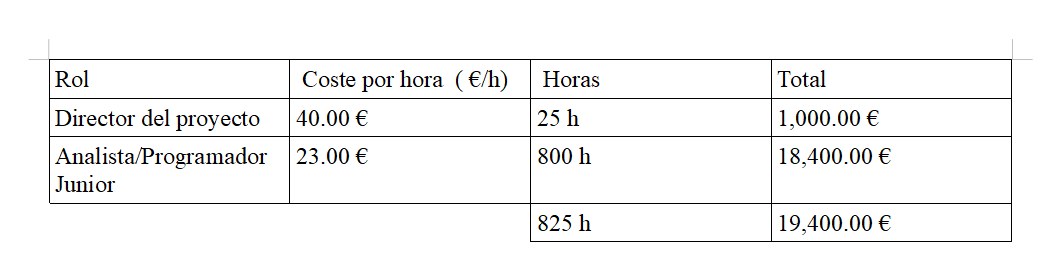
\includegraphics[width=0.75\textwidth] {coste.png}
		\caption{Costes asociados a este proyecto }
	\end{figure}






\begin{itemize}
\item En el rol de director de proyecto estarían los que 
supervisan y evalúan el proyecto. En este caso Javier y Óscar realizarán este rol.

\item Analista/programador, en este rol estaría la persona encargada de las tareas de análisis, diseño, desarrollo y de la creación de las pruebas para este proyecto. Al estar realizado por mi yo haría de este rol.





\end{itemize}
\section{Seguimiento}

Como se comentó a lo largo de este capítulo la metodología usada será  Scrum y el proyecto será dividido en Sprints de 4 semanas cada uno. El numero de Sprint que estimamos sería de 10.




 Antes de empezar con los Sprint comenzamos creando el Product Backlog. Ésto es más una lista con todas las funcionalidades del la aplicación priorizadas de más a menos importancia para nuestro proyecto. 

\subsection{Sprint 1}

En este primer Sprint nos centraremos en las tareas relacionadas con la capa intermedia. Para ello comenzamos diseñando la base de datos y modelo de datos, algo fundamental en cualquier aplicación para no heredar carencias en capas superiores. Posteriormente los servicios necesarios para el servicio REST.


\subsection{Sprint 2}
 Una vez implementado el servicio Rest, el objetivo en este Sprint será hacer las pruebas para él.
 Una vez acabas las pruebas el siguiente paso dentro de esté Sprint será la creación de las maquetas que servirán para la capa de presentación/cliente, es decir, el interface del usuario. Estas maquetas se irán revisando y refinando a lo largo del proyecto.
 
\subsection{Sprint 3}

En este Sprint se comenzará con el desarrollo de la aplicación Android. Comenzaremos permitiendo que el usuario sea capaz que conocer su localización dentro del mapa y que al ir desplazándose cambie su ubicación como también obtener las coordenadas de su posición. Este punto será básico para el resto de la aplicación ya nos proporciona los datos necesarios para guardar puntos y rutas. Los casos de uso realizados son los siguientes:

\begin{itemize}

\item\textbf{\textit{ R-PDI-1 Guardar Punto De Interés caza}}
\item\textit{ \textbf{R-PDI-2 Guardar Punto De Interés pesca}}
\item \textbf{\textit{R-PDI-3 Eliminar PDI}}
\item \textbf{\textit{R-PDI-4 Buscar los PDI}}
\end{itemize} 



\subsection{Sprint 4}

En este Sprint nos centraremos en el registro de usuarios y gestión parcial de grupos.



\begin{itemize}
\item\textbf{ \textit{R1}  Registrarse en la aplicación.}
\item \textbf{\textit{R2} Iniciar sesión en la aplicación. }
\item\textbf{ \textit{R-G-1 Crear grupo}}
\item\textbf{\textit{ R-G-2 Añadir integrantes}}
\end{itemize} 

\subsection{Sprint 5}
Este Sprint se centrará en acabar con la gestión de grupos.



\begin{itemize}
\item \textbf{\textit{R-G-3 Eliminar integrantes}},
\item \textbf{\textit{R-G-4 Ver grupos}}.
\item \textbf{\textit{R-G-5 Ver integrantes grupo}}

\end{itemize}

Además en este Sprint hemos desarrollado un toolbar para gestionar todas las opciones y mejorar la navegación del usuario en la aplicación.


\begin{figure}[H]
		\centering
		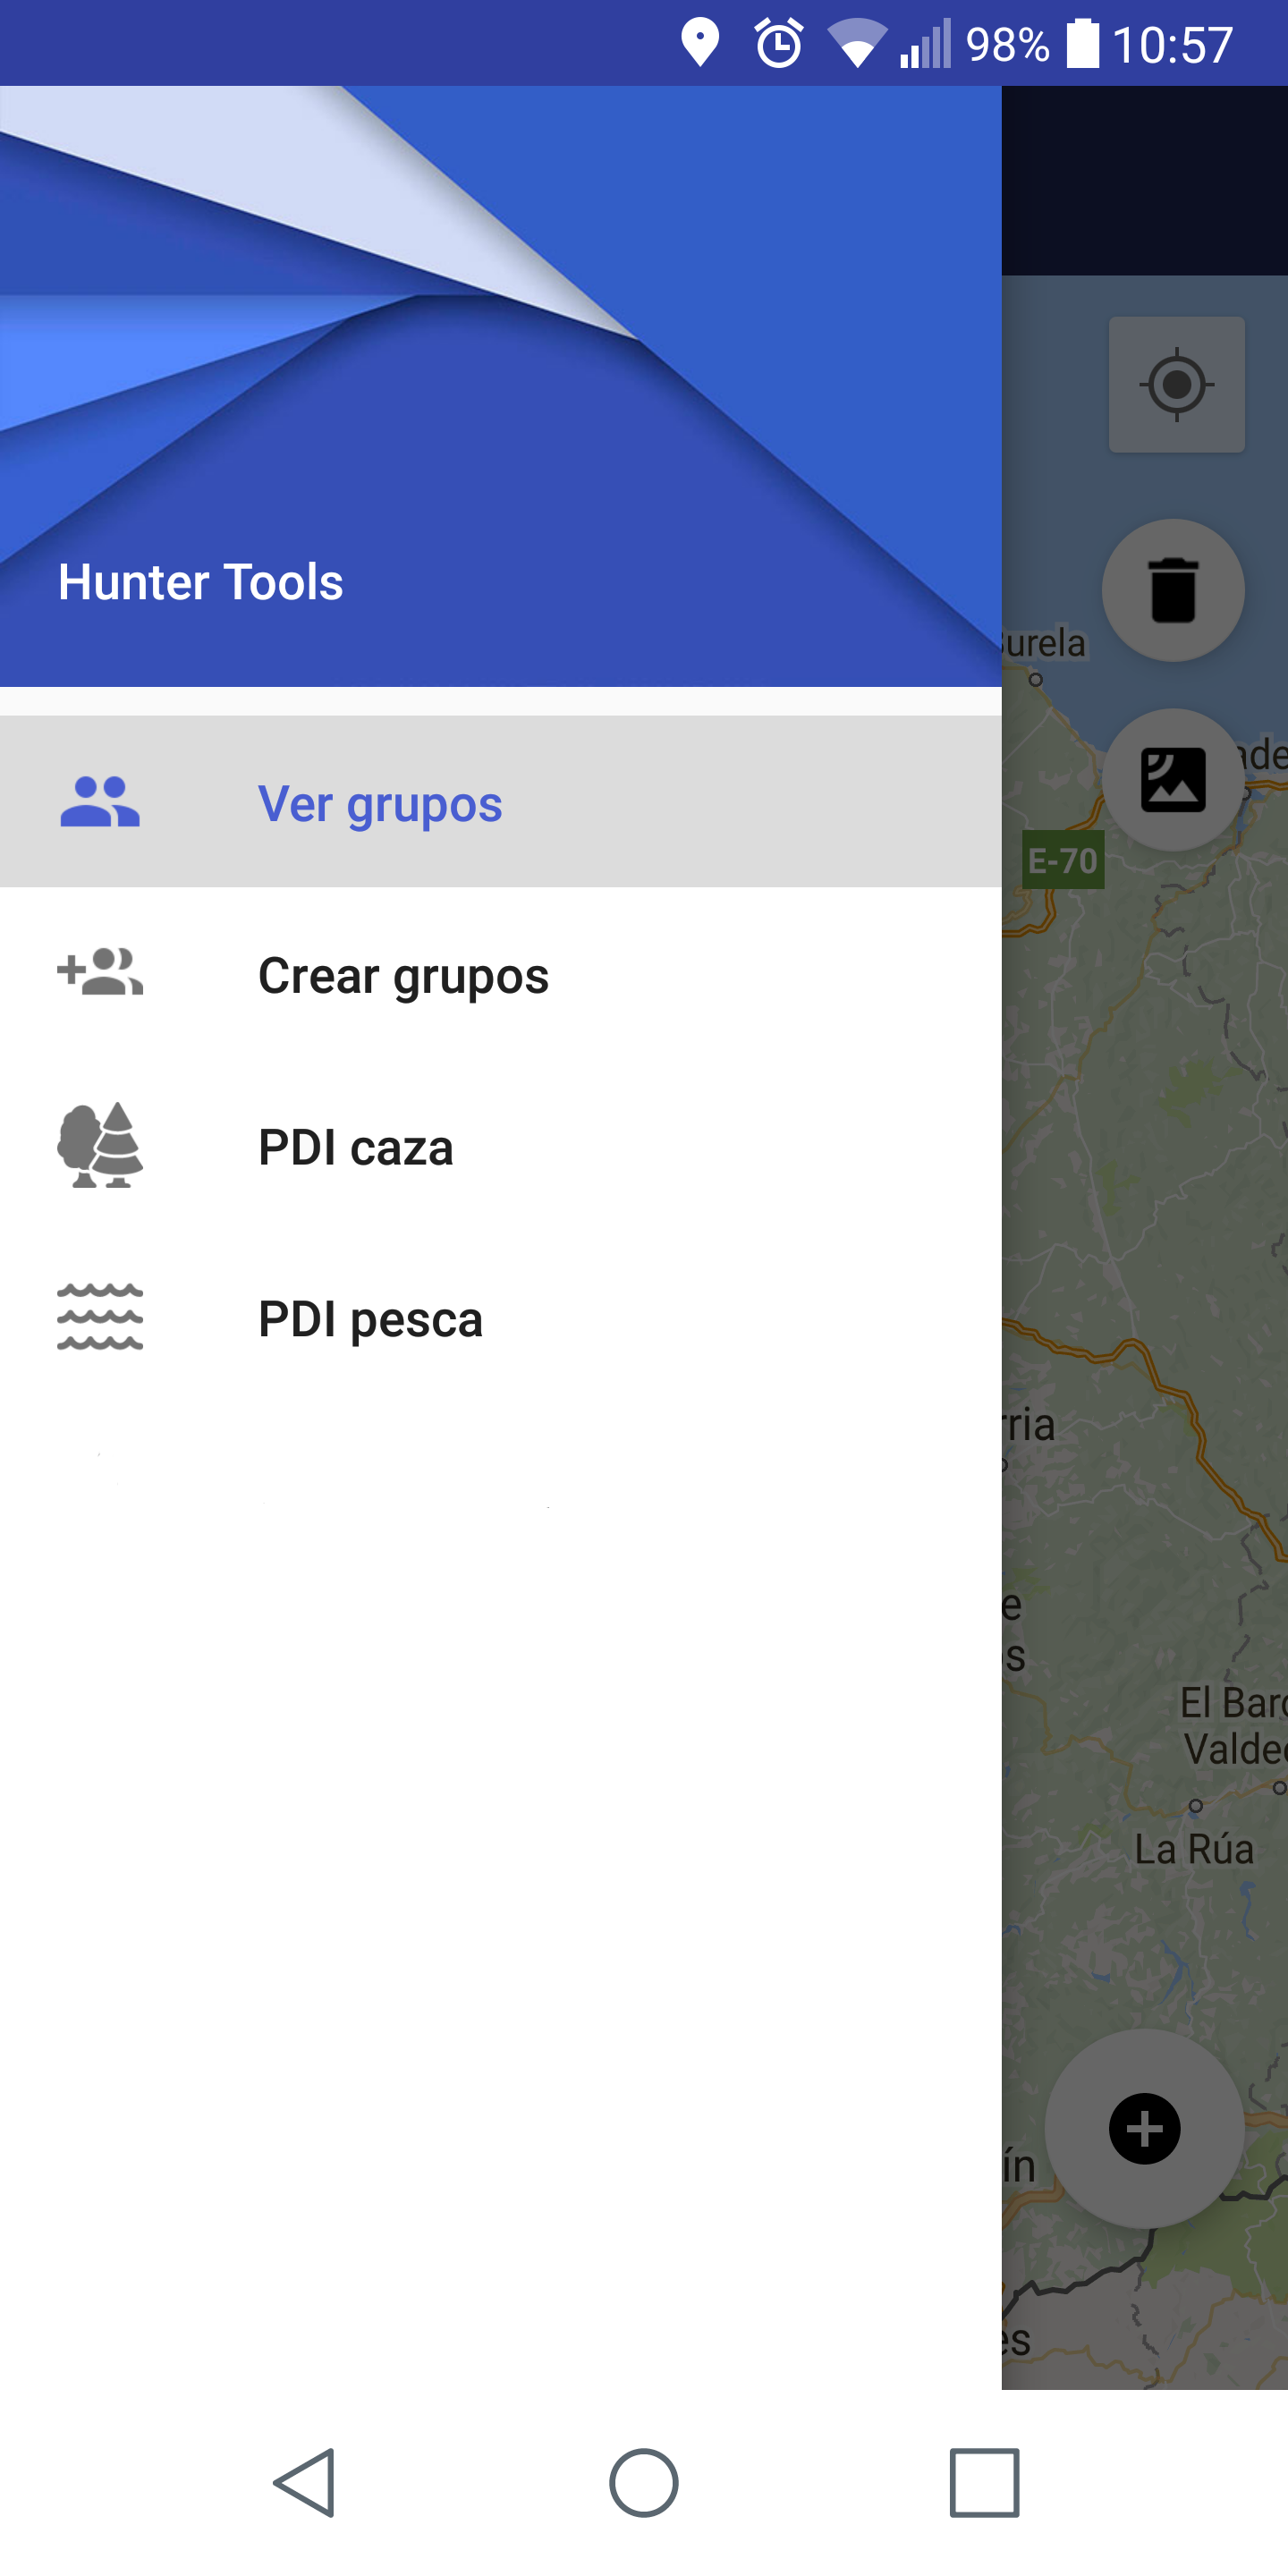
\includegraphics[width=0.5\textwidth] {menu.png}
		\caption{Captura del menú de navegación}
	\end{figure}

\subsection{Sprint 6}
\subsection{Sprint 7}
\subsection{Sprint 8}





\chapter{Diseño}
		

En este capítulo se comentará el diseño de la arquitectura general, el
modelo de datos y también aspectos más concretos del diseño del servidor y da aplicación
móvil.



\section{Esquema general de la arquitectura}
La aplicación que estamos desarrollando seguirá la arquitectura
en tres capas. Este patrón arquitectónico cliente/servidor se diferencian tres
capas, una capa de interface de usuario , una capa de persistencia
y una capa intermedia llamada de servicios que permite la llamada de forma remota a la capa modelo(capa que contiene la lógica) por parte del cliente. Este esquema esta compuesto por:




\begin{figure}[H]
		\centering
		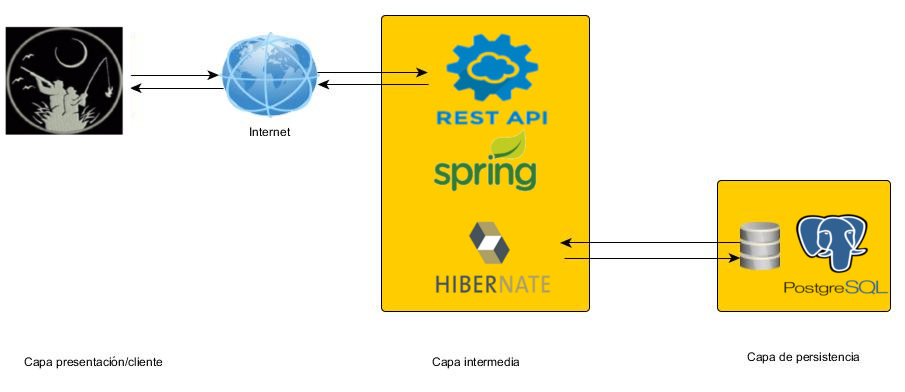
\includegraphics[width=0.75\textwidth] {arquitectura2.png}
		\caption{Esquema general de la arquitectura del sistema }
	\end{figure}


\begin{itemize}
\item \textbf{Capa de presentación/cliente}:\\
Capa que nos proporciona la información relacionada con los servicios que puede invocar el cliente. Es la encargada de comunicarse con las otras capas para guardar la información de cada usuario. En si es la capa con la que va a interactuar el usuario cada vez trabaje con esta aplicación.

\item \textbf{Capa intermedia:}\\
Esta capa es la encargada de enlazar la capa de persistencia con la capa de presentación/cliente. Lo que hace es recoger los datos que provienen de la base de datos, necesarios para satisfacer el servicio invocado y enviárselos al cliente.

\item \textbf{Capa de persistencia:}\\
Esta capa es la encargada de almacenar los datos del sistemas en la base de datos, además contiene todos los mecanismos de acceso a datos necesarios para poder hacer persistentes los datos.
 Esta capa debe ofrecer una interface que ayude a la comunicación con la capa intermedia, de manera que se abstraiga de la tecnología usada en el sistema de almacenamiento y no cree una dependencia con ella. Esta abstracción permitirá hacer cambios o actualizaciones en la tecnología sin afectar a otras capas con las que pudiera interaccionar en un futuro.\\
 


\end{itemize}
Un vez comentada la arquitectura general del sistema, pasaremos a comentar la capa intermedia un poco más a fondo ya que en ciertas ocasiones, la capa intermedia puede estar compuesta de N-capas(Arquitectura en N-capas). Ésta es una de esas ocasiones.

Los servidores que siguen el modelo Modelo-Vista-Controlador consiguen separar los datos de la  aplicación, la lógica de negocio  y el envío  de información por la red.
Ésta separación ayuda al desarrollo de la aplicación tanto a la hora de crear la como a la hora de hacer su mantenimiento ya que marca al desarrollador a colocar el código en una capa concreta. \\


Los componentes capas que componen al patrón MVC son:

\begin{itemize}
\item \textbf{Modelo:}
Está compuesta por clases que tienen acceso a los datos ofreciendo unos métodos para ser usados de manera sencilla por las capas superiores. Éstos métodos son los encargados de acceder a la base de datos y proporcionar los datos persistentes.
\item \textbf{Vista:}
Esta formada por el interfaz donde se realizan las llamadas entre el servicio web, peticiones HTTP en las que la información va en formato JSON, y la aplicación cliente.
\item \textbf{Controlador:}
Esta capa será la encargada de implementar la lógica del interface llamando a las operaciones que ofrece el modelo y seleccionando la vista asociada a cada petición.
\end{itemize}
\begin{figure}[H]
		\centering
		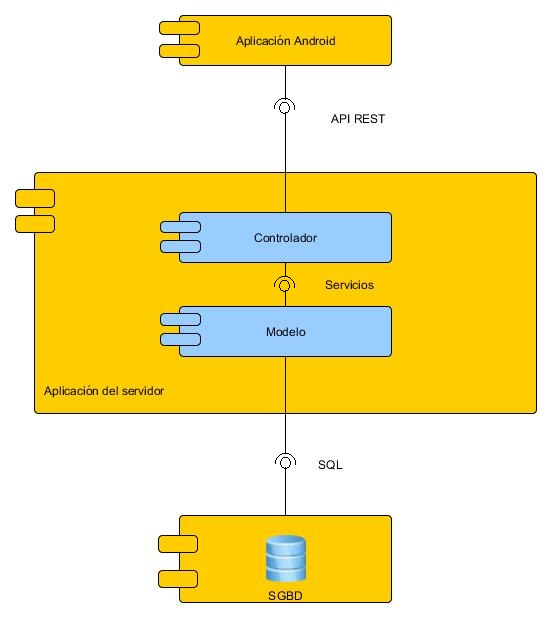
\includegraphics[width=0.75\textwidth] {componentes.jpg}
		\caption{Diagrama de componentes del sistema }
	\end{figure}

\section{Modelo de datos}
\begin{figure}[H]
		\centering
		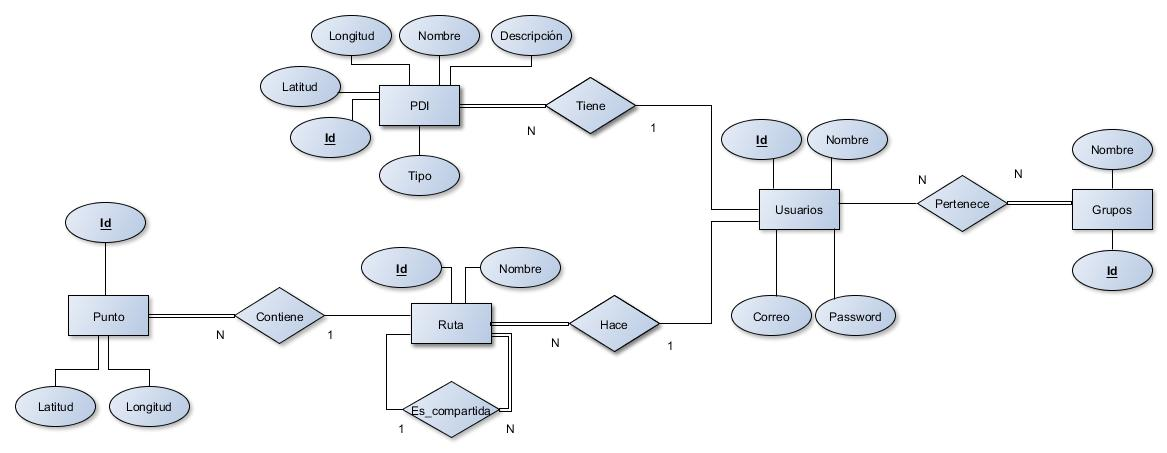
\includegraphics[width=0.95\textwidth] {BD.jpg}
		\caption{Entidad relación  }
	\end{figure}
\section{Servidor}
Para permitir una comunicación entre la aplicación del cliente y la capa de persistencia hemos desarrollado un servidor desplegado en un proveedor de servidores , al que se podrá acceder de manera remota y que permitirá tener acceso a las funcionalidades de la capa persistente.

La solución mencionada anteriormente será un servidor, en java, que  usará Spring ya que facilita la creación de aplicaciones de forma cómoda y rápida.\\

Durante el desarrollo de este proyecto el servidor ha sido desplegado en un proveedor de servidores virtuales llamado 
  DigitalOcean, ya que ofrece distintos lugares donde poder ubicar lo hemos decidido hacerlo en uno concreto de Alemania para que el ping fuera más cercano y rápido.
\begin{figure}[H]
		\centering
		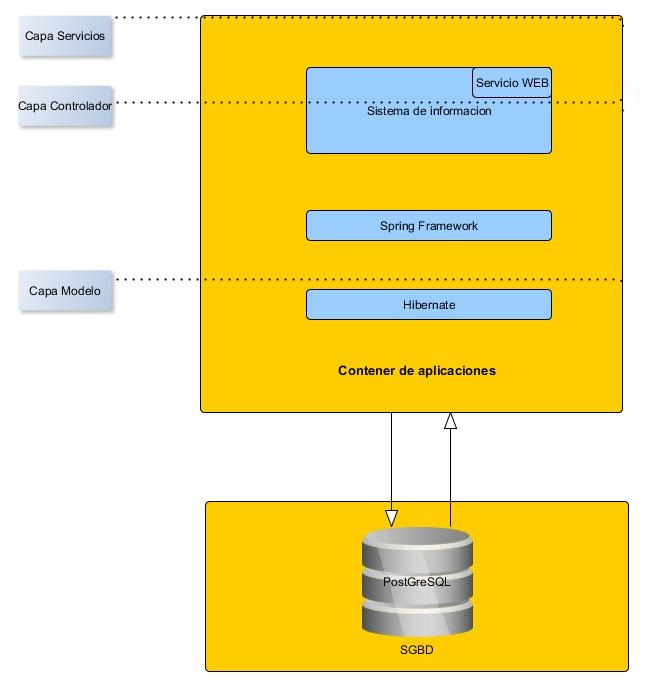
\includegraphics[width=0.75\textwidth] {arquitectura-servidor.jpg}
		\caption{Arquitectura del servidor }
	\end{figure}


\subsection{Servicio web}
 La comunicación en esta capa se hará mediante una API. Una API describE la forma en que los programas o los sitios webs intercambian datos, cuyo formato  de intercambio de datos normalmente es JSON. En este servicio hemos decidido usar una API REST, un tipo de arquitectura de desarrollo web que se apoya totalmente en el estándar HTTP para la obtención de datos. A través de los siguientes peticiones podremos acceder a los distintos recursos.
 

\begin{itemize}
\item Los métodos de acceso indican la acción se queremos realizar sobre los recursos de nuestro sistema. Siguiendo esta linea tenemos el GET para solicitar un recurso pedido. POST para crear el recurso en el sistema y  para eliminar recursos usaremos DELETE. 



\item Dependiendo del método usado se irán cambiando la ruta en la petición HTTP y el contenido de ellas(cuerpo). Un POST tendrá una URL sencilla ya que los datos del objetos para ser creado irán en el cuerpo mientras que el GET y DELETE la tendrán de la forma \textit{ /usuario/{idusuario}} para obtener un objeto concreto o eliminarlo.





 


\end{itemize}

\subsection{Organizacion dos paquetes}
A aplicación del servidor sigue un arquetipo en 5 paquetes distintos de clases Java y uno para los test:
\subsubsection{java}
\begin{itemize}
\item\textbf{ es.udc.fi.dc.config} Contiene las clases Java de configuración de Spring.
\item \textbf{es.udc.fi.dc.model} Contiene todos los modelos de datos que estarán almacenados en la base de datos.
\item \textbf{es.udc.fi.dc.daos} Contiene los interfaces (JpaRepository) que aceden a los datos del sistema.
\item \textbf{es.udc.fi.dc.controller} Contiene as clases relacionadas  con las peticiones remotas.
\item  \textbf{es.udc.fi.dc.services} Contiene tanto los interfaces de los servicios como la implementación de los mismos.


\end{itemize}
\subsubsection{test}

\textbf{es.udc.fi.dc.test} Contiene las clases que realizan los test.
\subsection{Transmisión de la información}
Como se mencionó anteriormente para el servicio web usaremos la API REST, esta necesita un lenguaje de intercambio para la transmisión de información. El formato que seguiremos para la transmisión será el JSON y como parseador Jackson.
JSON, siglas JavaScript Object Notation, es un formato estándar de transmisión de la información muy cómodo de usar que emplea pares de clave-valor.
	\begin{figure}[H]
		\centering
		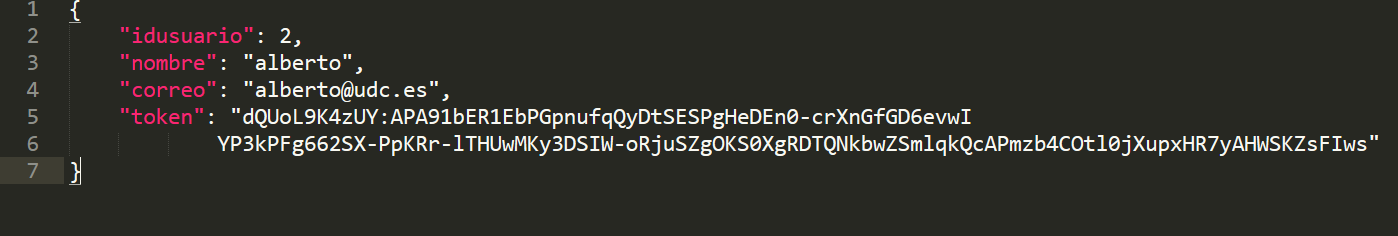
\includegraphics[width=0.5\textwidth] {json.PNG}
		\caption{JSON }
	\end{figure}
\subsection{Gestión de las clases persistentes}
Para gestionar las clases persistentes de nuestro aplicación usaremos el patrón de diseño basado en DAO(Data Access Object).

 Un DAO define un interfaz que contiene conjunto de operaciones de persistencia y a su vez una implementacion permitiendo la gestión de las entidades en la base de datos. Es decir oculta la gestión de la base de datos y a su vez la tecnología que usamos en ella, dotando a cada clase persistente de un DAO asociado a ella. En éste proyecto hemos usado Spring Data JPA que nos proporciona una interfaz para la gestión de los objetos del dominio sin tener que escribir nosotros la implementacion de los métodos. Esto nos permite ganar agilidad a la hora de crear los DAOs ya que permite extender esta interfaz a nuestra clase DAO proporcionando todos los métodos CRUD, métodos para modificar o eliminar objetos de ese tipo. Éste interfaz se llama JpaRepository.\\


Otro motivo por el cual usamos JpaRepository es que permite extender la creación de una buena seria de métodos de búsqueda por el nombre de los atributos de nuestras clases persistentes simplemente definiendo los como un método de nuestro interfaz del DAO.
	\begin{figure}[H]
		\centering
		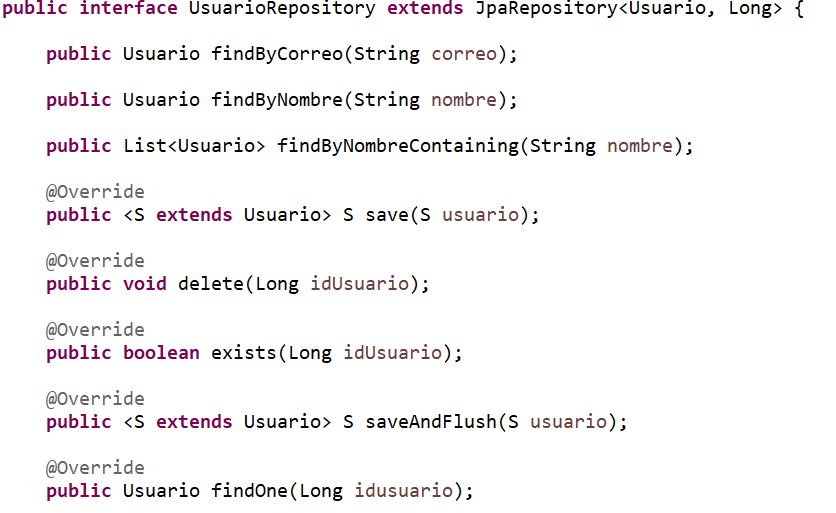
\includegraphics[width=0.75\textwidth] {jparepository.PNG}
		\caption{Ejemplo de interfaz con JpaRepository }
	\end{figure}
\section{Aplicación Móvil}
La capa de presentación será accesible por el usuario a través de una aplicación móvil desarrollada en Android. Los aspectos más relevantes serán expuestos a continuación.

\subsection{Servicios}
\begin{itemize}
\item \textbf{Google Maps API}. Es un servicio web proporcionado por google que nos permite usar los mapas en nuestras aplicaciones y también conocer la ubicación del usuario  en todo momento. Esta ubicación la marca con un punto azul pero no suministra coordenadas(latitud y longitud).
\item \textbf{Google Location}. Es un servicio de google que nos suministra las coordinadas del usuario, según varia la posición ciertos metros o cada cierto tiempo.
\item \textbf{Rest SystemService}. Este punto seria el que ejecuta nuestro propio servidor para guardar o devolver lo datos de los usuario, puntos de interés, rutas o grupos del usuario.
\item \textbf{Firebase Cloud Messaging} Firebase Cloud Messaging (FCM) es una solución de mensajería multiplataforma que te permite enviar mensajes de forma segura y gratuita. En este caso lo hemos utilizado para enviar notificaciones push cuando se inicia una ruta compartida.
\end{itemize}
\begin{figure}[H]
		\centering
		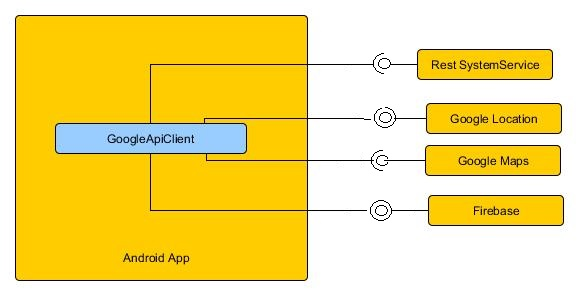
\includegraphics[width=0.75\textwidth] {arquitectura-movil.jpg}
		\caption{Servicios de la aplicación móvil }
	\end{figure}
	
	
\subsection{Organización de los paquetes}
La organización seguida en la aplicación móvil es la de agrupar las clases por funcionalidades comunes.
\begin{itemize}
\item  \textbf{com.example.alberto.hunter-android.activities}, contiene todas las actividades.
\item \textbf{com.example.alberto.hunter-android.adapter}, contiene los adaptadores.
\item \textbf{com.example.alberto.hunter-android.model},contiene todos los modelos de datos.
\item \textbf{com.example.alberto.hunter-android.utils}, contiene las clases auxiliares.\\ 

Con esta organización por funcionalidades comunes creamos un proyecto claro y  organizado lógicamente.

\end{itemize}



 		


\chapter{Implementación}
		
\section{Implementación}
En este capítulo expondremos la implementacion tanto del servidor como de la aplicación móvil.


\subsection{Servidor}
En capítulos anteriores ya comentamos la estructura de paquetes seguida para desarrollar el servidor, en este hablaremos de JpaRepository.\\

JpaRepository es un repositorio que nos ofrece métodos genéricos de gestión de clases persistentes como también métodos mas concreto que nos permiten realizar operaciones complejas abstrayendonos de su implementacion.

Ademas este repositorio se adapta a la clase con la que va a trabajar.
\begin{figure}[H]
		\centering
		
\includegraphics[width=\textwidth] {jpa.png}
		\caption{UsuarioRepository}
		\label{fig:jpa}
	\end{figure}
	



\begin{lstlisting}[language=java,
 ,backgroundcolor=\color{backcolour},   
    commentstyle=\color{codegreen},
    keywordstyle=\color{magenta},
    numberstyle=\tiny\color{codegray},
    stringstyle=\color{codepurple}]
  @Autowired
	private UsuarioService usuarioService;

	@Autowired
	private GrupoService grupoService;

	@Test
	public void testprueba() {
\end{lstlisting}
	
Como se puede ver en la figura anterior, este interfaz importa la clase Usuario accediendo a todos sus atributos y generando una lista de métodos para estos atributos concretos como podemos ver en la siguiente.
\begin{figure}[H]
		\centering
		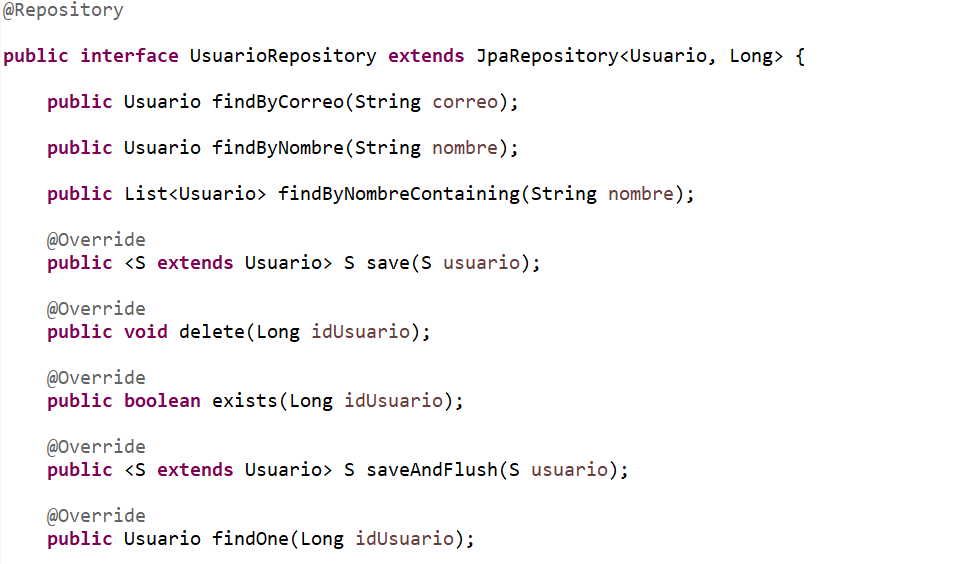
\includegraphics[width=\textwidth] {jpa2.png}
		\caption{UsuarioRepository métodos}
	\end{figure}


\newpage

 
 
 
 
 \subsection{Aplicación móvil Android}
En este capítulo comentaremos aspectos concreto de la implementación de de la aplicación móvil.



\subsubsection{Mapas}

 Para la creación de rutas tanto individuales como compartidas como para crear PDI el usuario necesita conocer las coordenadas de los puntos por lo que trascurre su ruta. Para ello necesitamos los mapas de Google Maps y métodos de sus APIs.
 
 
 \begin{lstlisting}[language=java,
 ,backgroundcolor=\color{backcolour},   
    commentstyle=\color{codegreen},
    keywordstyle=\color{magenta},
    numberstyle=\tiny\color{codegray},
    stringstyle=\color{codepurple}]
compile 'com.google.android.gms:play-services-maps:10.2.0'

\end{lstlisting}
 
 Con la dependencia de la figura anterior permitimos a nuestra aplicación que use los servicios de  Google Maps.\\
 Para marcar un punto en el mapa y que este quede visible en el mapa necesitamos implementar un método que capture los clic en el mapa y que nos devuelva las coordenadas del punto marcado.
 
 
 \begin{lstlisting}[language=java,
 ,backgroundcolor=\color{backcolour},   
    commentstyle=\color{codegreen},
    keywordstyle=\color{magenta},
    numberstyle=\tiny\color{codegray},
    stringstyle=\color{codepurple}]
    
mMap.setMyLocationEnabled(true);
mMap.getUiSettings().setCompassEnabled(true);
mMap.setOnMapClickListener(new GoogleMap
	.OnMapClickListener() {
	public void onMapClick(LatLng point) {
	mMap.clear();
	poilongitud = point.longitude;
	poilatitud = point.latitude;
	LatLng Yo = new LatLng(poilatitud, poilongitud);
	Marker mensaje = 
	mMap.addMarker(new MarkerOptions()
		.position(Yo)
		.title("Guardar este punto?"));
  	mensaje.showInfoWindow();
	VerTodosPois();

\end{lstlisting} 
 
 
 
 
  Con el fragmento de código de la figura anterior  se capturaría ese clic y aparecería el Marker común de todos los mapas de Google Maps acompañado del mensaje \textit{"Guardar este punto?"}. En nuestro proyecto personalizamos los Marker de modo que cuando guardamos ese punto pase a a representarse con icono de un pescador o de un cazador dependiendo del PDI que estuviéramos guardando. Para ello usamos el siguiente fragmento de código.

 

\begin{lstlisting}[language=java,
 ,backgroundcolor=\color{backcolour},   
    commentstyle=\color{codegreen},
    keywordstyle=\color{magenta},
    numberstyle=\tiny\color{codegray},
    stringstyle=\color{codepurple}]
    
protected Marker createMarkerPesca(double
		latitude,Double longitude, String nombre,
		String	descripcion) {
       		return mMap.addMarker(new MarkerOptions()
                	.position(new LatLng(latitude, 							longitude))
                	.anchor(0.5f, 0.5f)
                	.title(nombre).snippet(descripcion)
	                .icon(BitmapDescriptorFactory
    	       		.fromResource(R.drawable.pescador)));
    }


\end{lstlisting} 
 
 
 
 Y así es como quedaría.  

 
 
 
	\begin{figure}[H]
\begin{minipage}[b]{0.5\linewidth} %Una minipágina que cubre la mitad de la página
\centering
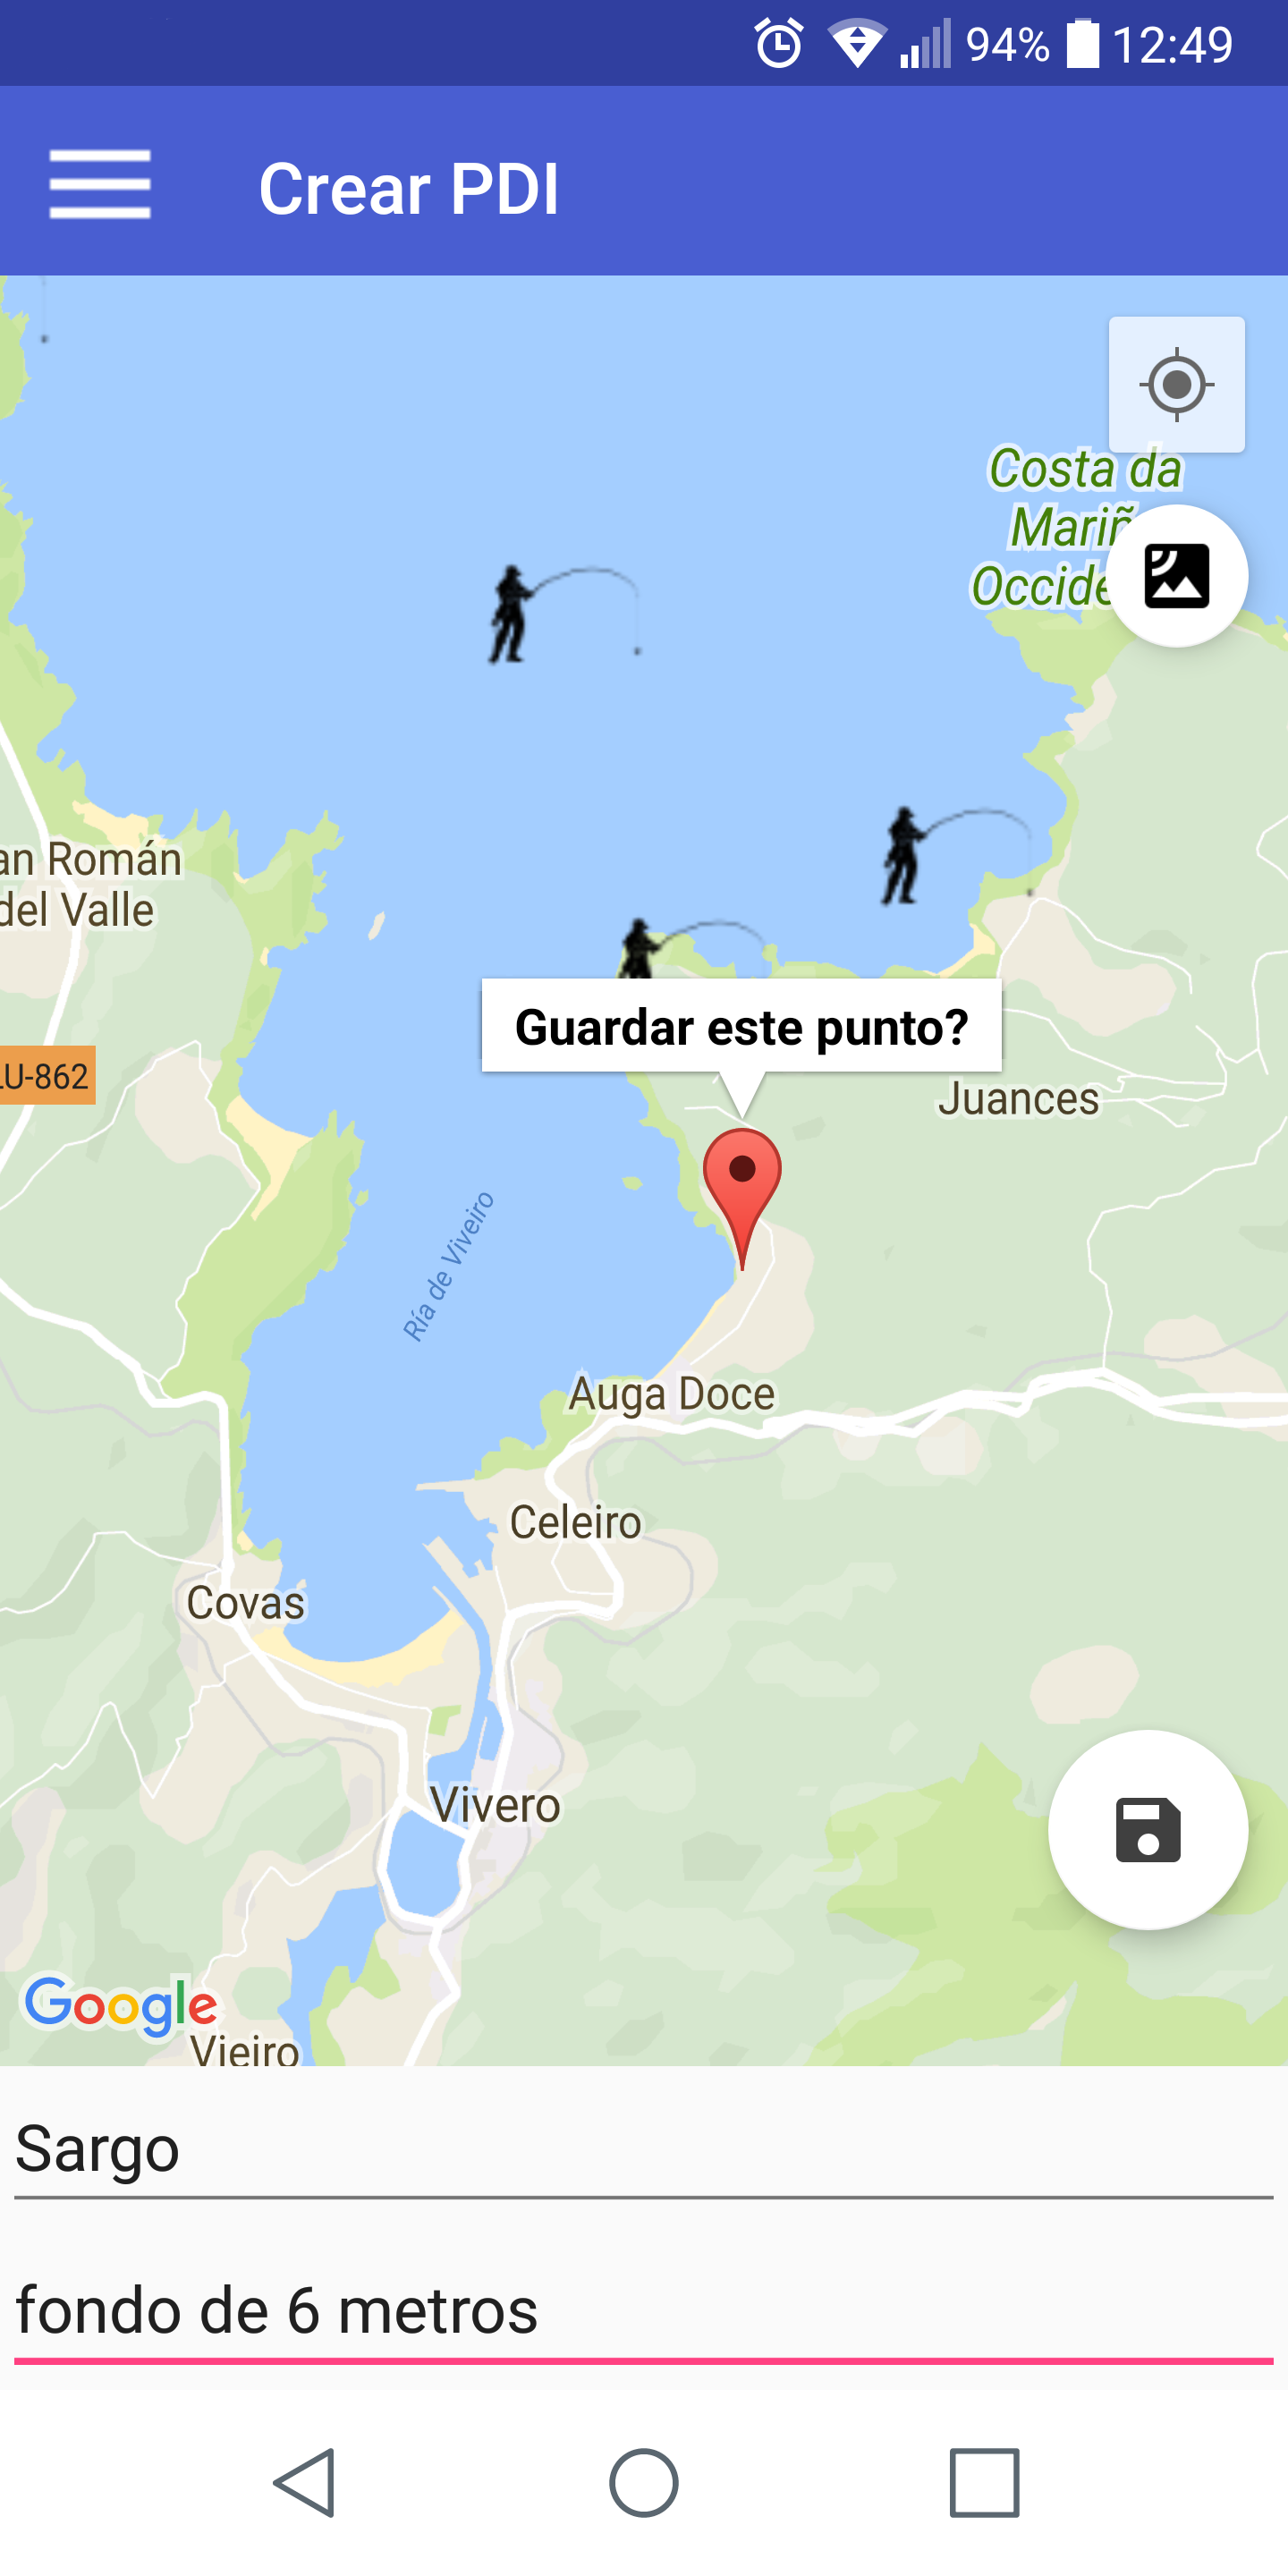
\includegraphics[width=6cm]{capturamovil/pdiguardar.png}
 \label{figura1}
\caption{Marker antes de guardar el PDI}

\end{minipage}
\hspace{0.5cm} % Si queremos tener un poco de espacio entre las dos figuras
\begin{minipage}[b]{0.5\linewidth}
\centering
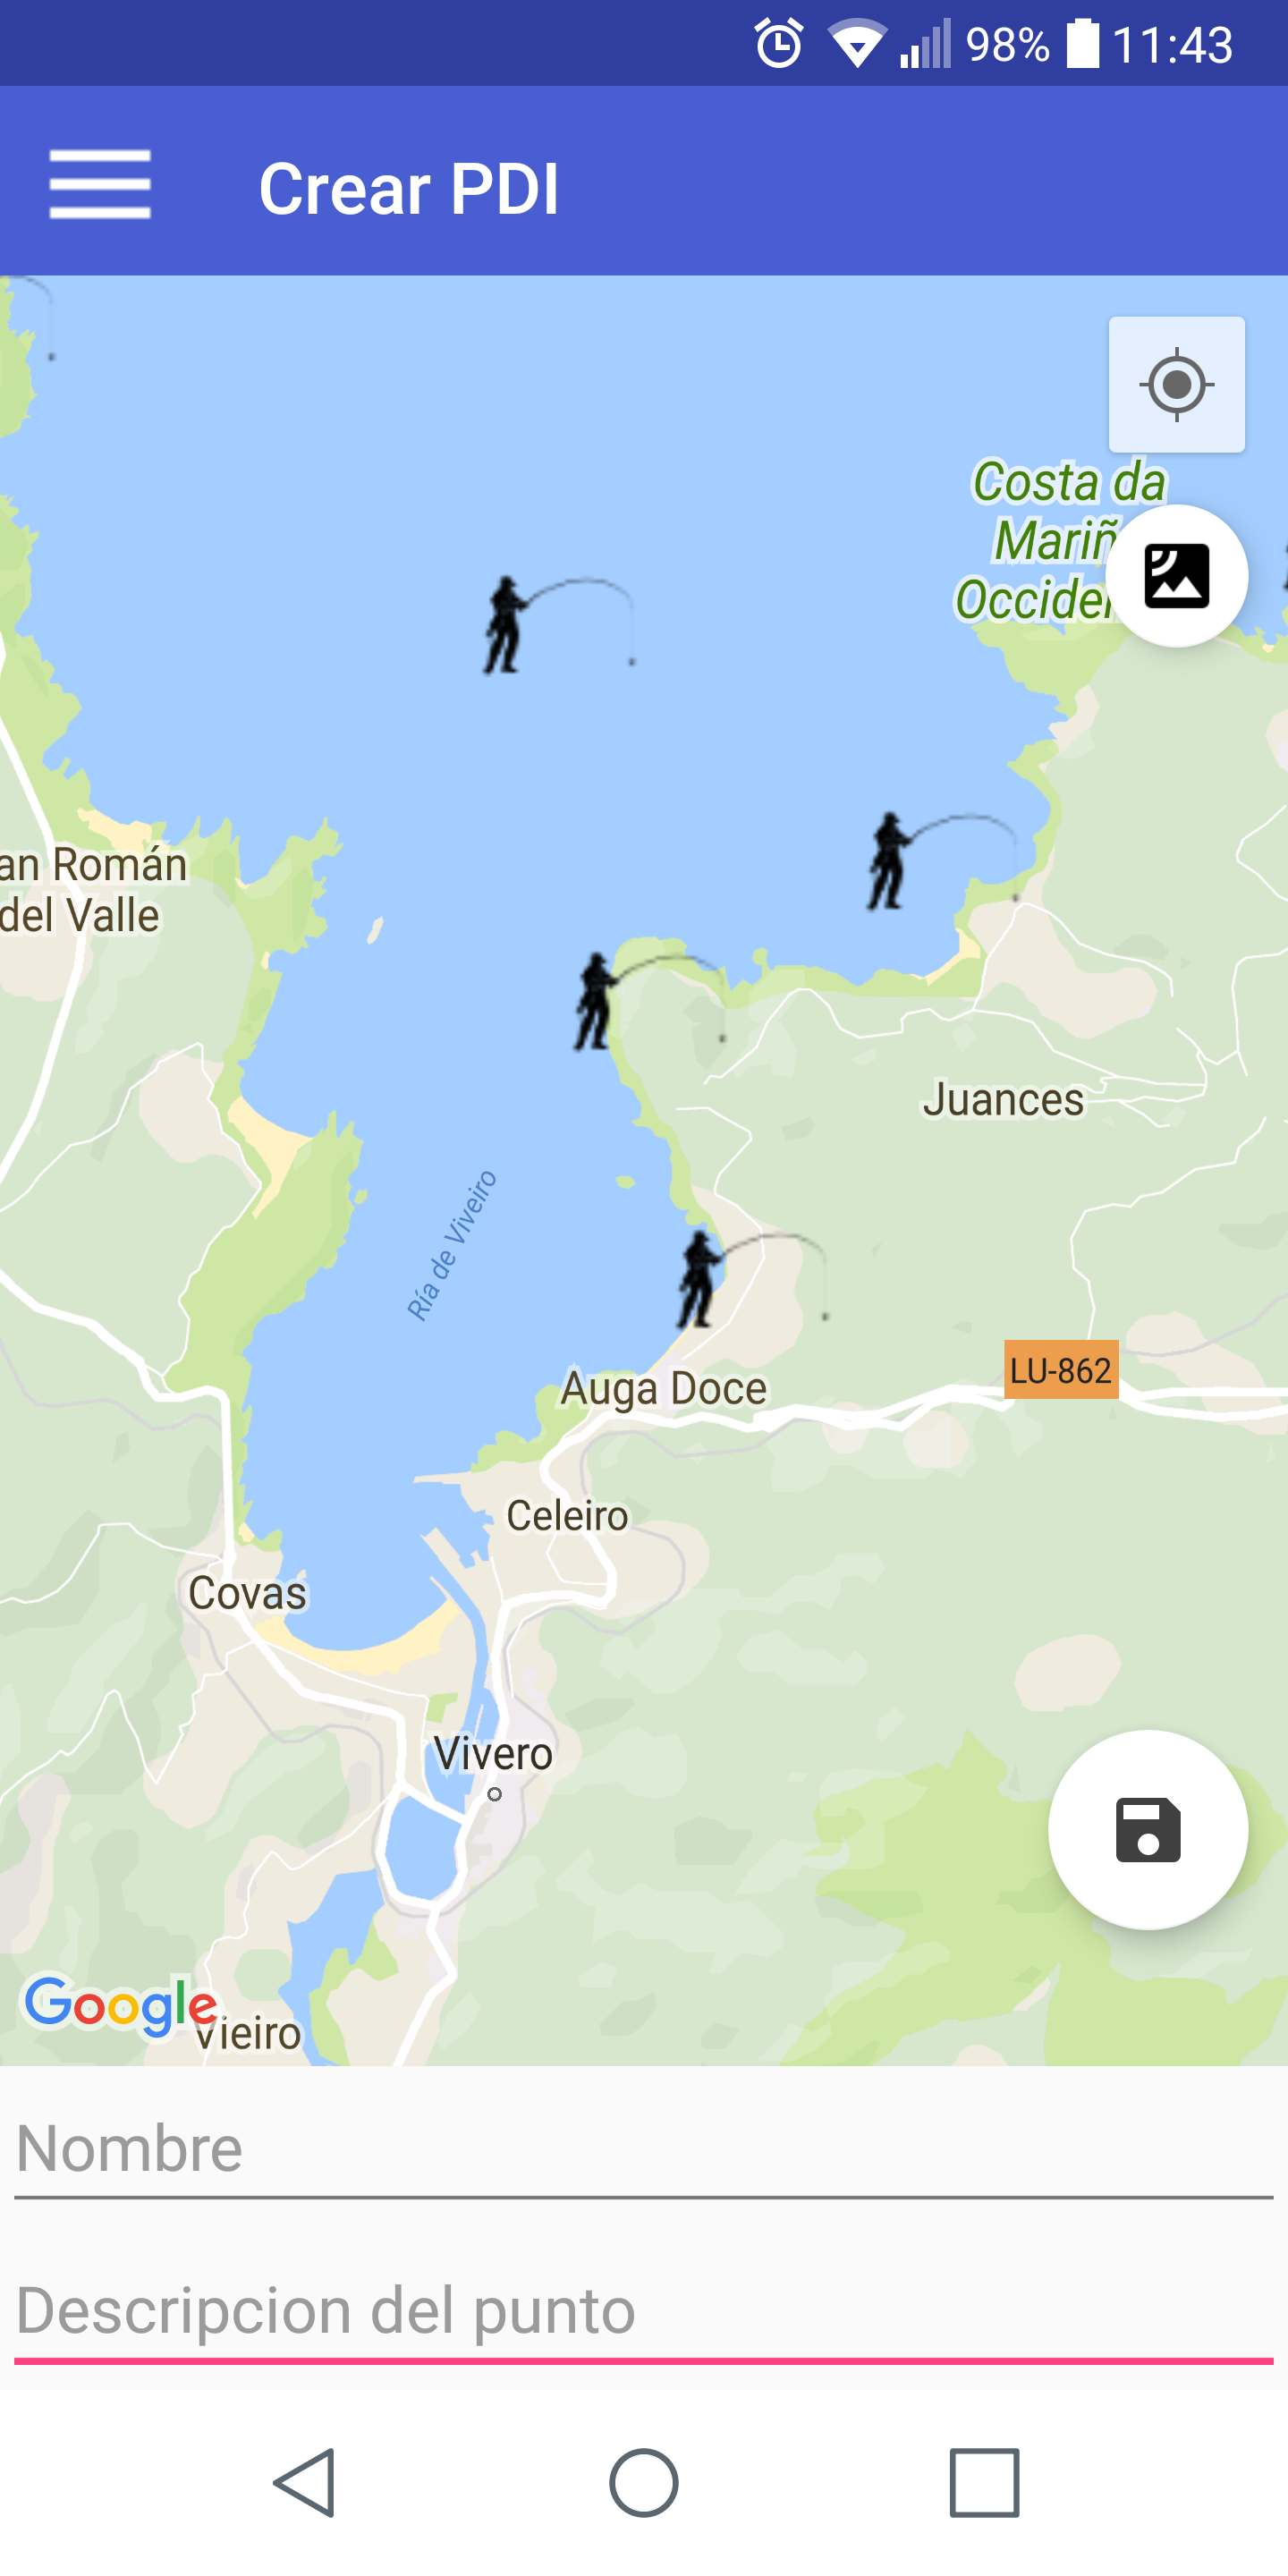
\includegraphics[width=6cm]{capturamovil/pdiguardar2.png}
 \label{figura2}
\caption{Marker después }

\end{minipage}
\end{figure} 
 
 
 
 \subsubsection{Localización}
  Para la creación de ruta necesitamos una método que nos proporcione las coordenadas(latitud y longitud) de los puntos por los que trascurre el usuario en la ruta. Para ellos necesitamos la siguiente dependencia.

	
\begin{lstlisting}[language=java,
 ,backgroundcolor=\color{backcolour},   
    commentstyle=\color{codegreen},
    keywordstyle=\color{magenta},
    numberstyle=\tiny\color{codegray},
    stringstyle=\color{codepurple}]
compile 'com.google.android.gms:play-services-location:10.2.0'


\end{lstlisting}	
	
	
	Una vez añadida esta dependencia necesitamos un método que nos proporciones las coordenadas concretas, para ellos usaremos el siguiente fragmento de código.
	
\begin{lstlisting}[language=java,
 ,backgroundcolor=\color{backcolour},   
    commentstyle=\color{codegreen},
    keywordstyle=\color{magenta},
    numberstyle=\tiny\color{codegray},
    stringstyle=\color{codepurple}]
mlocManager.requestLocationUpdates(LocationManager
.GPS_PROVIDER15, 0,(LocationListener) Local);


\end{lstlisting}	

El método ofrece el par de coordenadas cuando el usuario se mueve X metros o bien por un intervalo de tiempo en segundos.


Como se puede observar en la figura anterior en nuestro proyecto indicamos que los segundos que deberían transcurrir para devolver una coordenadas sería de 15.\\
Cuando nosotros estamos realizando la ruta en ocasiones el GPS pierde precisión y sitúa al usuario en punto un tanto lejano, lo cual es imposible ya que no se puede mover tan rápido. Este error del GPS lo hemos resuelto de la siguiente manera.

\begin{lstlisting}[language=java,
 ,backgroundcolor=\color{backcolour},   
    commentstyle=\color{codegreen},
    keywordstyle=\color{magenta},
    numberstyle=\tiny\color{codegray},
    stringstyle=\color{codepurple}]
      iniTramo = finTramo;
      finTramo = new LatLng(latitud, longitud);
      Location location1 = new Location("localizacion 1");
      location1.setLatitude(iniTramo.latitude);  //latitud
      location1.setLongitude(iniTramo.longitude); //longitud
      Location location2 = new Location("localizacion 2");
      location2.setLatitude(finTramo.latitude);  //latitud
      location2.setLongitude(finTramo.longitude); //longitud
      double distance = location1.distanceTo(location2);
\end{lstlisting}

En este código lo que hacemos es calcular la distancia entre dos puntos consecutivos. Este método pertenece a la API, para calcularla necesita el par de coordenadas y el ya se encarga de tener en cuenta la curvatura de la tierra para hacer la medición. Si esta distancia es superior a 15 metros desechamos ese punto.

\begin{figure}[H]
		\centering
		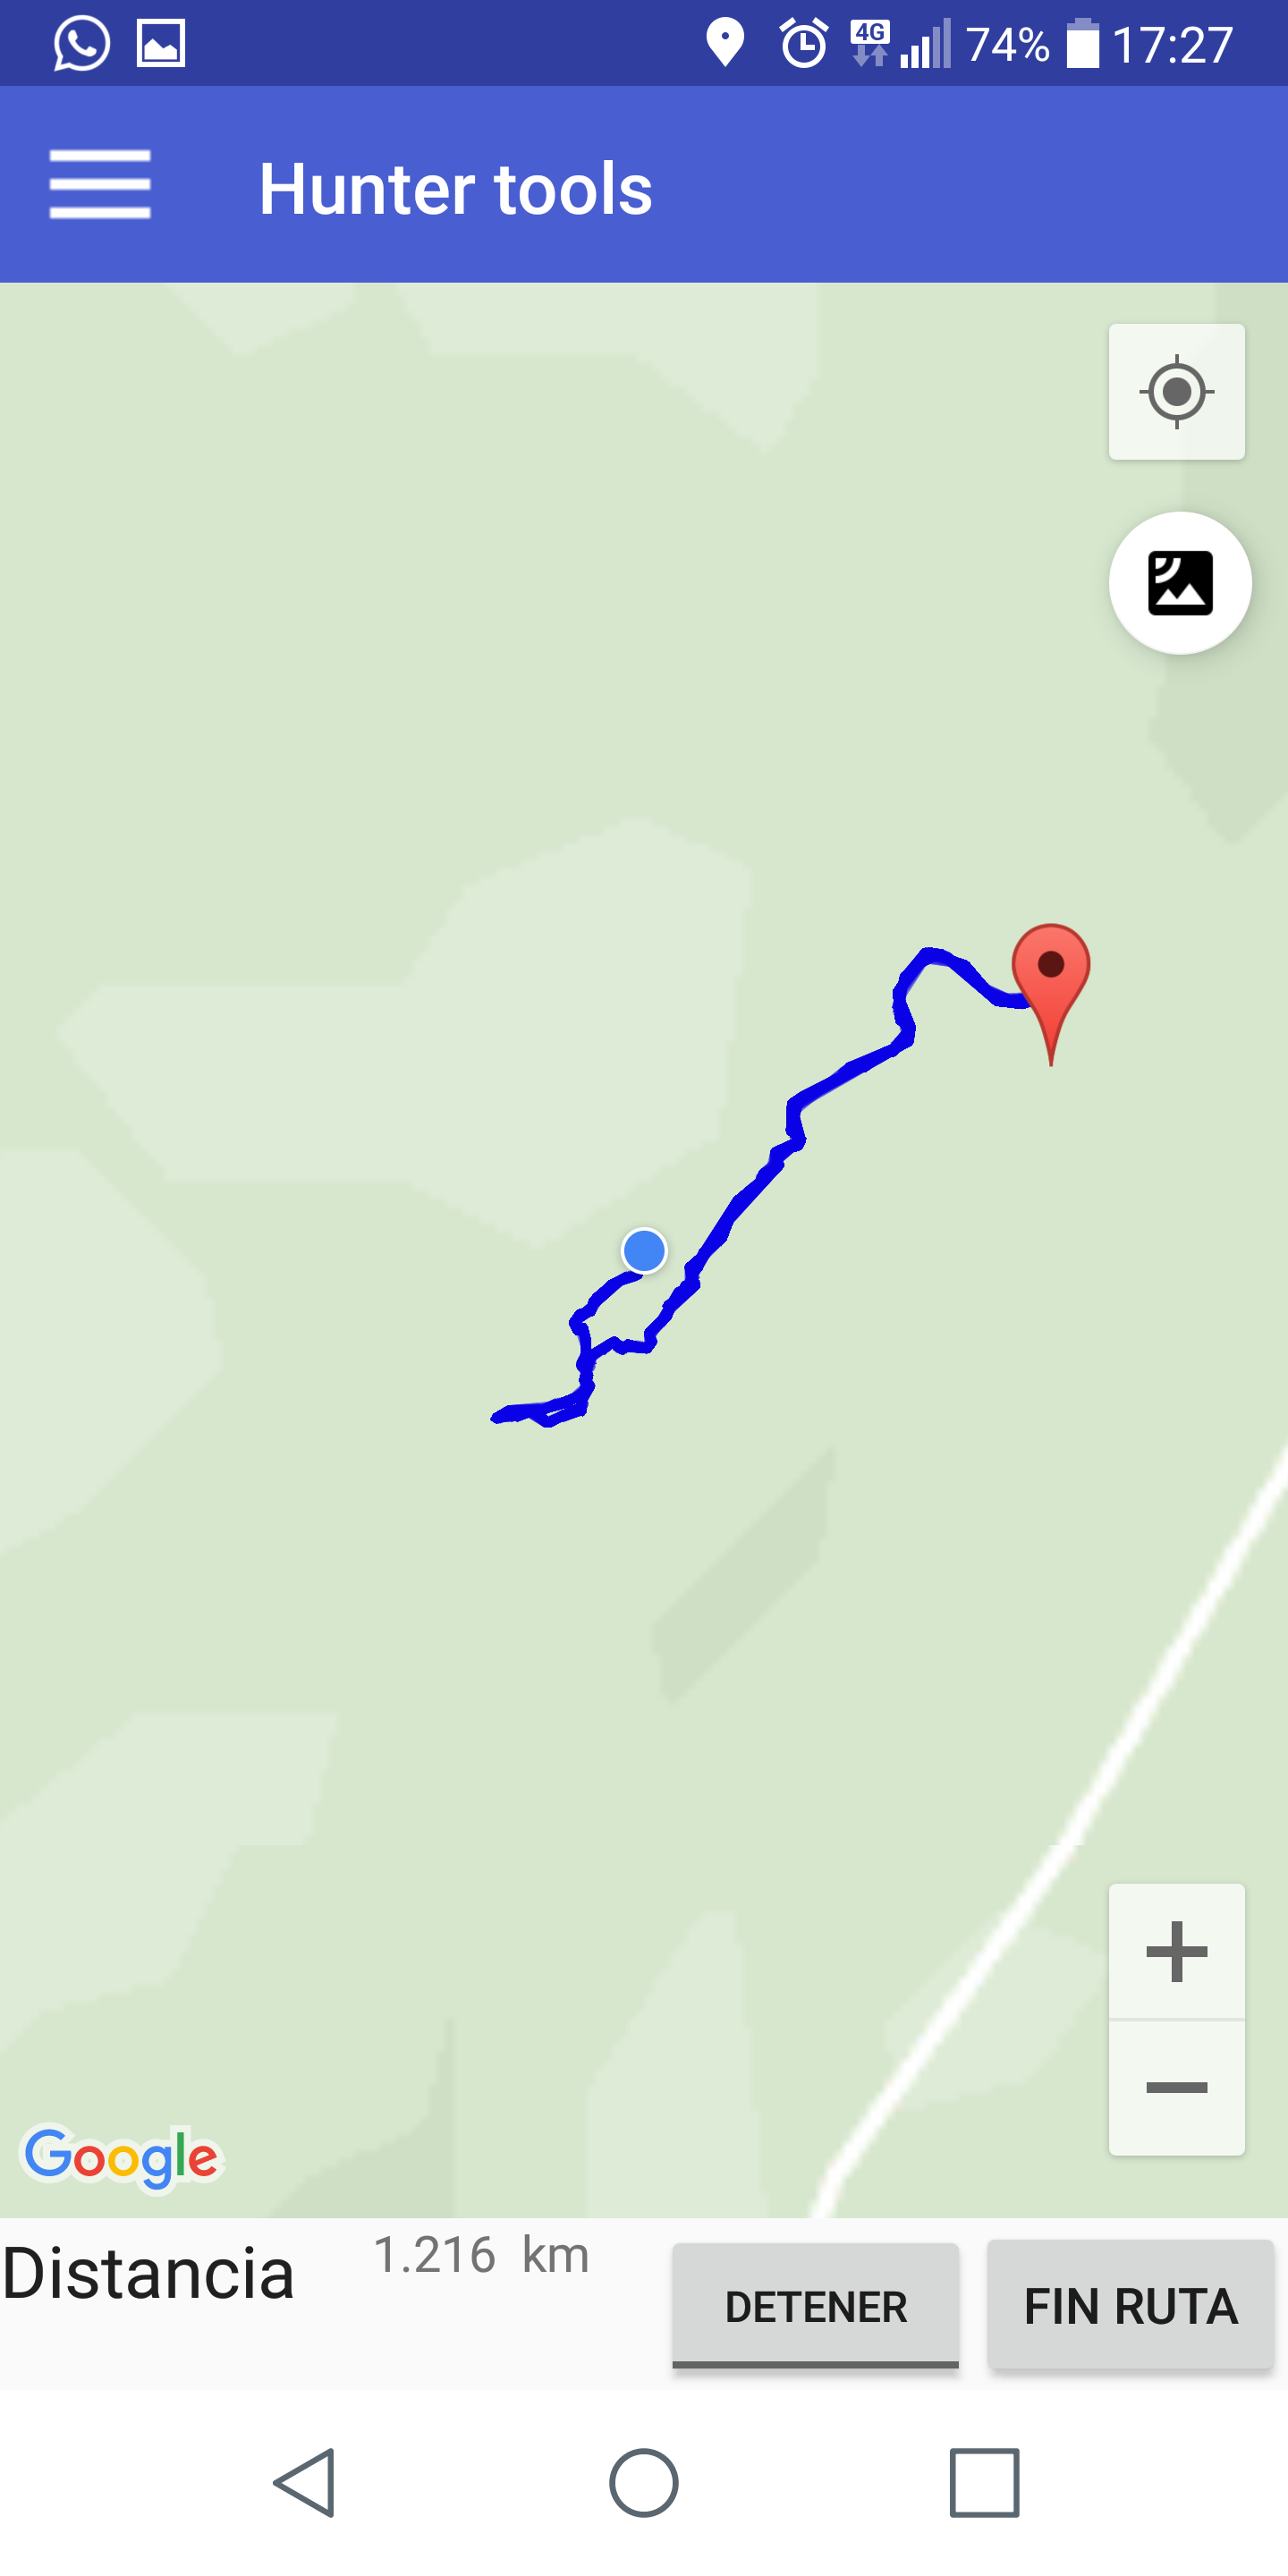
\includegraphics[width=0.4\textwidth] {capturamovil/individual-navegacion.png}
		\caption{Visualización de la ruta}
	\end{figure}
	
\subsubsection{Firebase} 
Cuando el usuario inicia una ruta compartida la forma en la que avisa al resto de usuario que la acaba de iniciar es mediante las Notificaciones Push con Firebase. Para ello tenemos que empezar añadiendo las dependencias siguientes.

	\begin{lstlisting}[language=java,
 ,backgroundcolor=\color{backcolour},   
    commentstyle=\color{codegreen},
    keywordstyle=\color{magenta},
    numberstyle=\tiny\color{codegray},
    stringstyle=\color{codepurple}]
 compile 'com.google.firebase:firebase-core:10.2.0'
 compile 'com.google.firebase:firebase-messaging:10.2.0'

\end{lstlisting}
	
Del lado del servidor enviamos una notificación con una serie de campos necesarios para identificar la ruta a un usuario concreto. Este usuario lo identificamos por un token que almacenamos en la base de dato, este token es característico de cada móvil. Para que nuestra aplicación  pueda recibir y entender esta notificación necesitaremos el siguiente fragmento de código.
	\begin{lstlisting}[language=java,
 ,backgroundcolor=\color{backcolour},   
    commentstyle=\color{codegreen},
    keywordstyle=\color{magenta},
    numberstyle=\tiny\color{codegray},
    stringstyle=\color{codepurple}]
 @Override
 public void onMessageReceived(RemoteMessage remoteMessage) {
        Map<String, String> data = remoteMessage.getData();
        titulo= data.get("titulo");
        nombreGrupo= data.get("nombreGrupo");
        accion= data.get("accion");
        idRuta= data.get("idRuta");
        verAccionString ();
        EventBus.getDefault().post(remoteMessage
        .getData().toString());
       
           }

\end{lstlisting}
Este método pasearía el JSON que envía el servidor y guardaría los datos necesario en el móvil.
En la siguiente captura veríamos la notificación en el móvil.	
	
	\begin{figure}[htbp]
\begin{minipage}[b]{0.5\linewidth} %Una minipágina que cubre la mitad de la página
\centering
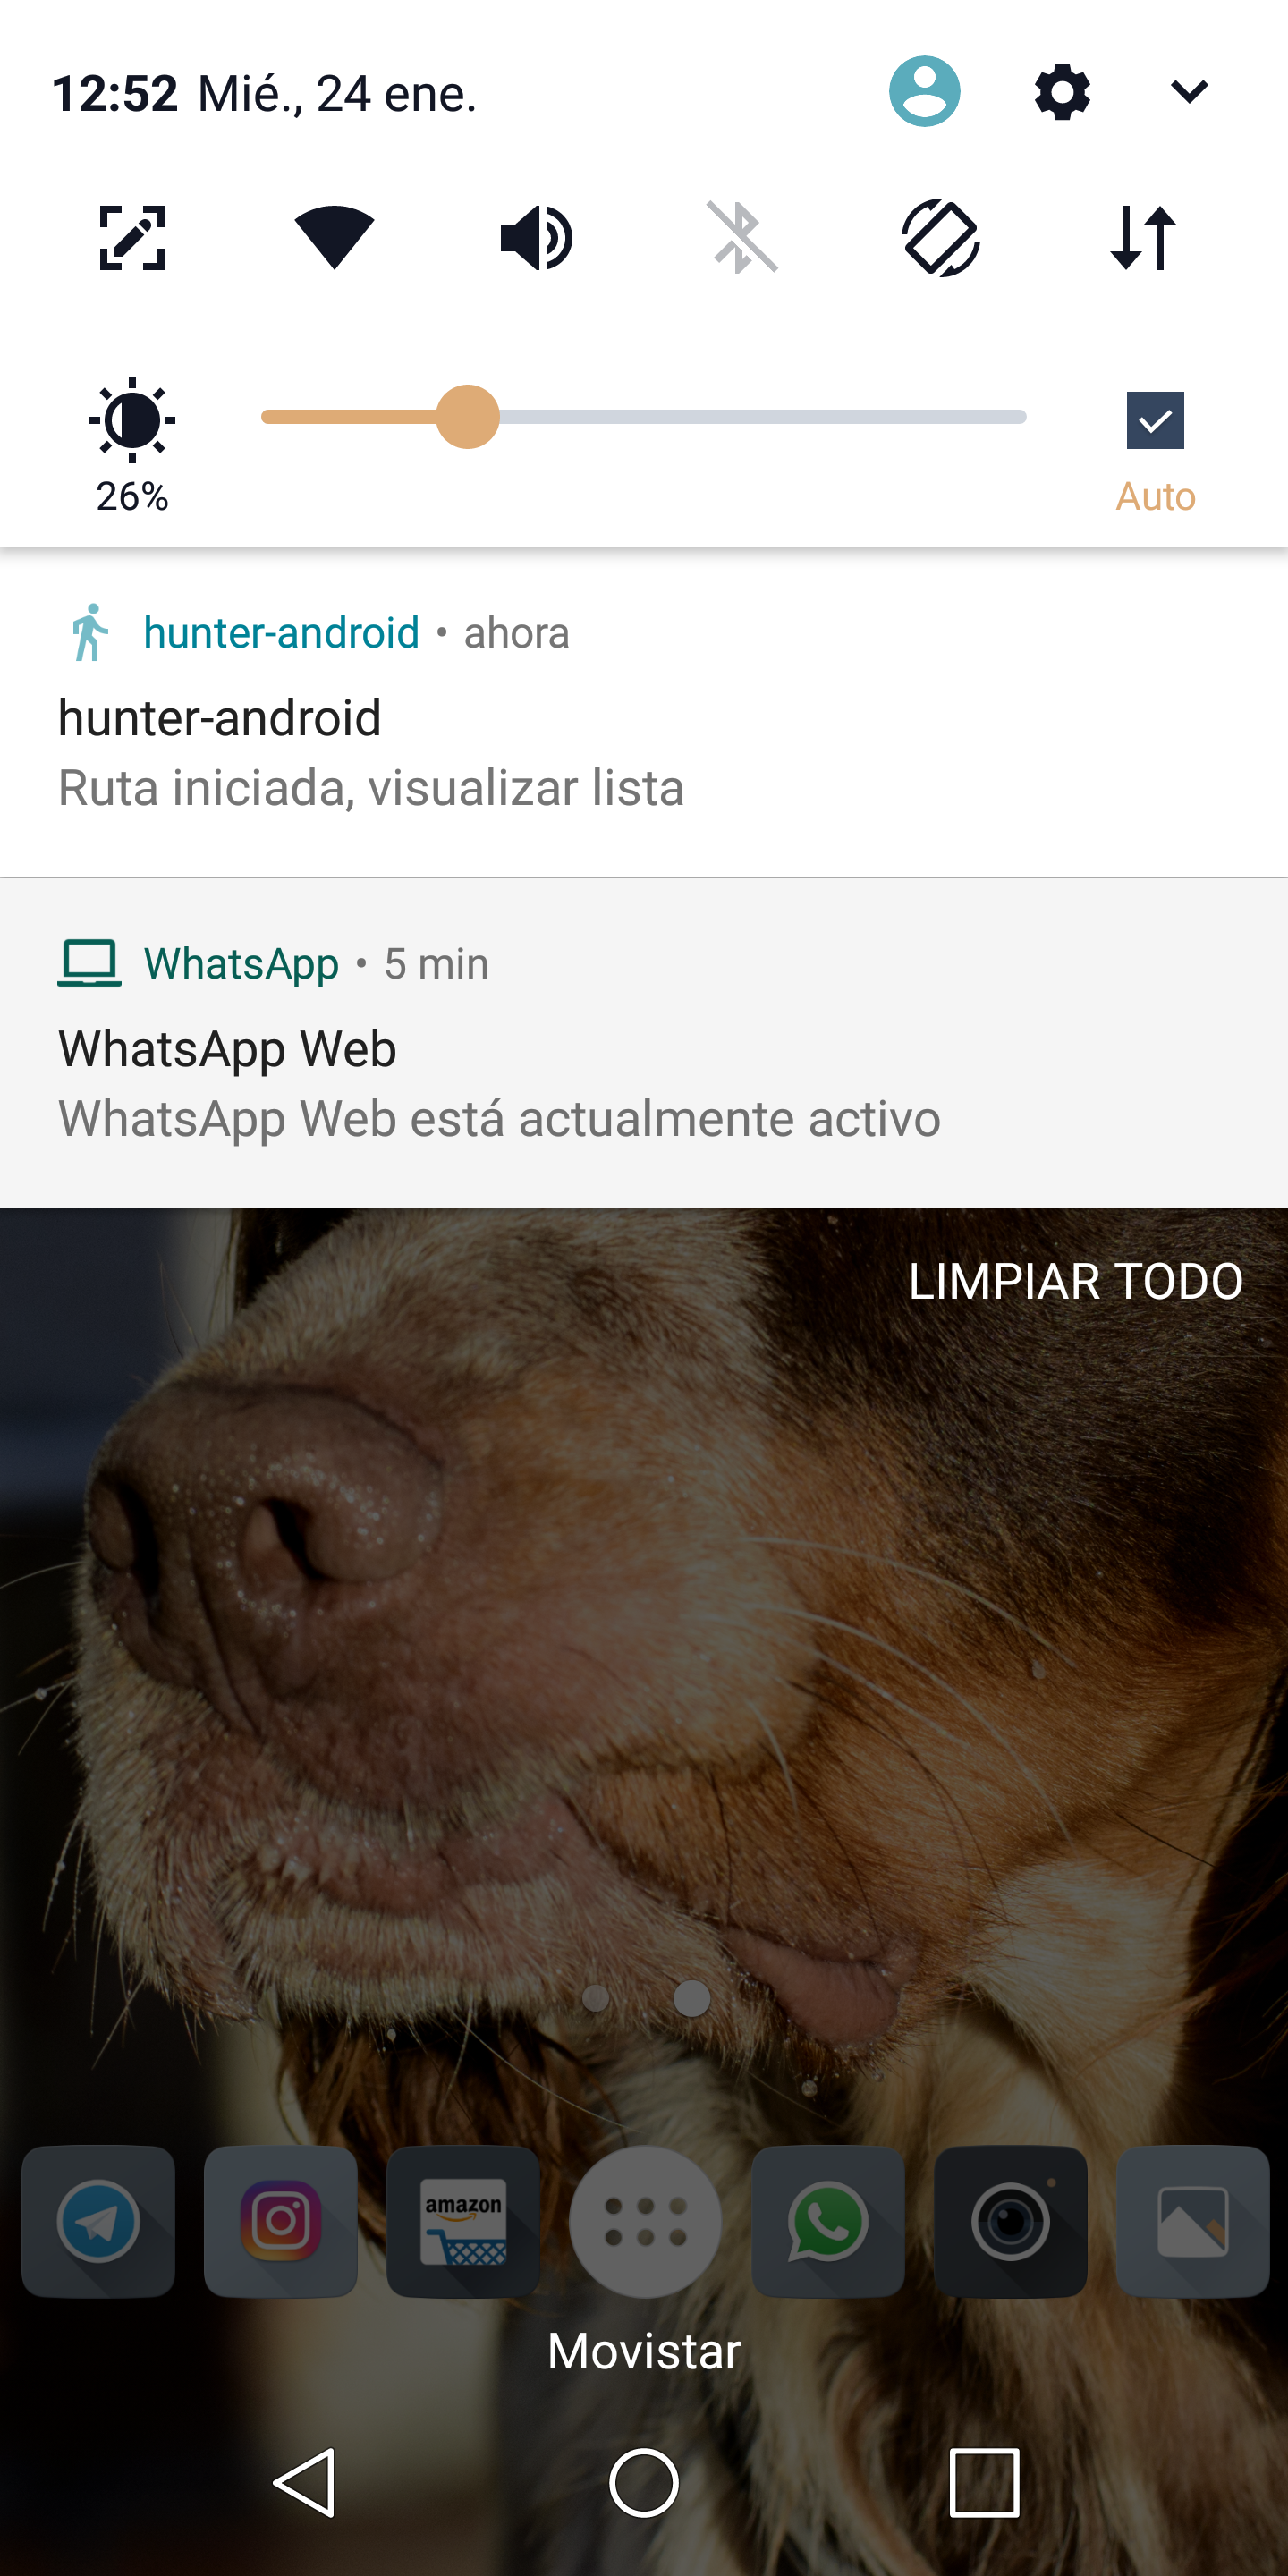
\includegraphics[width=6cm]{capturamovil/push1.png}
 \label{figura1}

\end{minipage}
\hspace{0.5cm} % Si queremos tener un poco de espacio entre las dos figuras
\begin{minipage}[b]{0.5\linewidth}
\centering
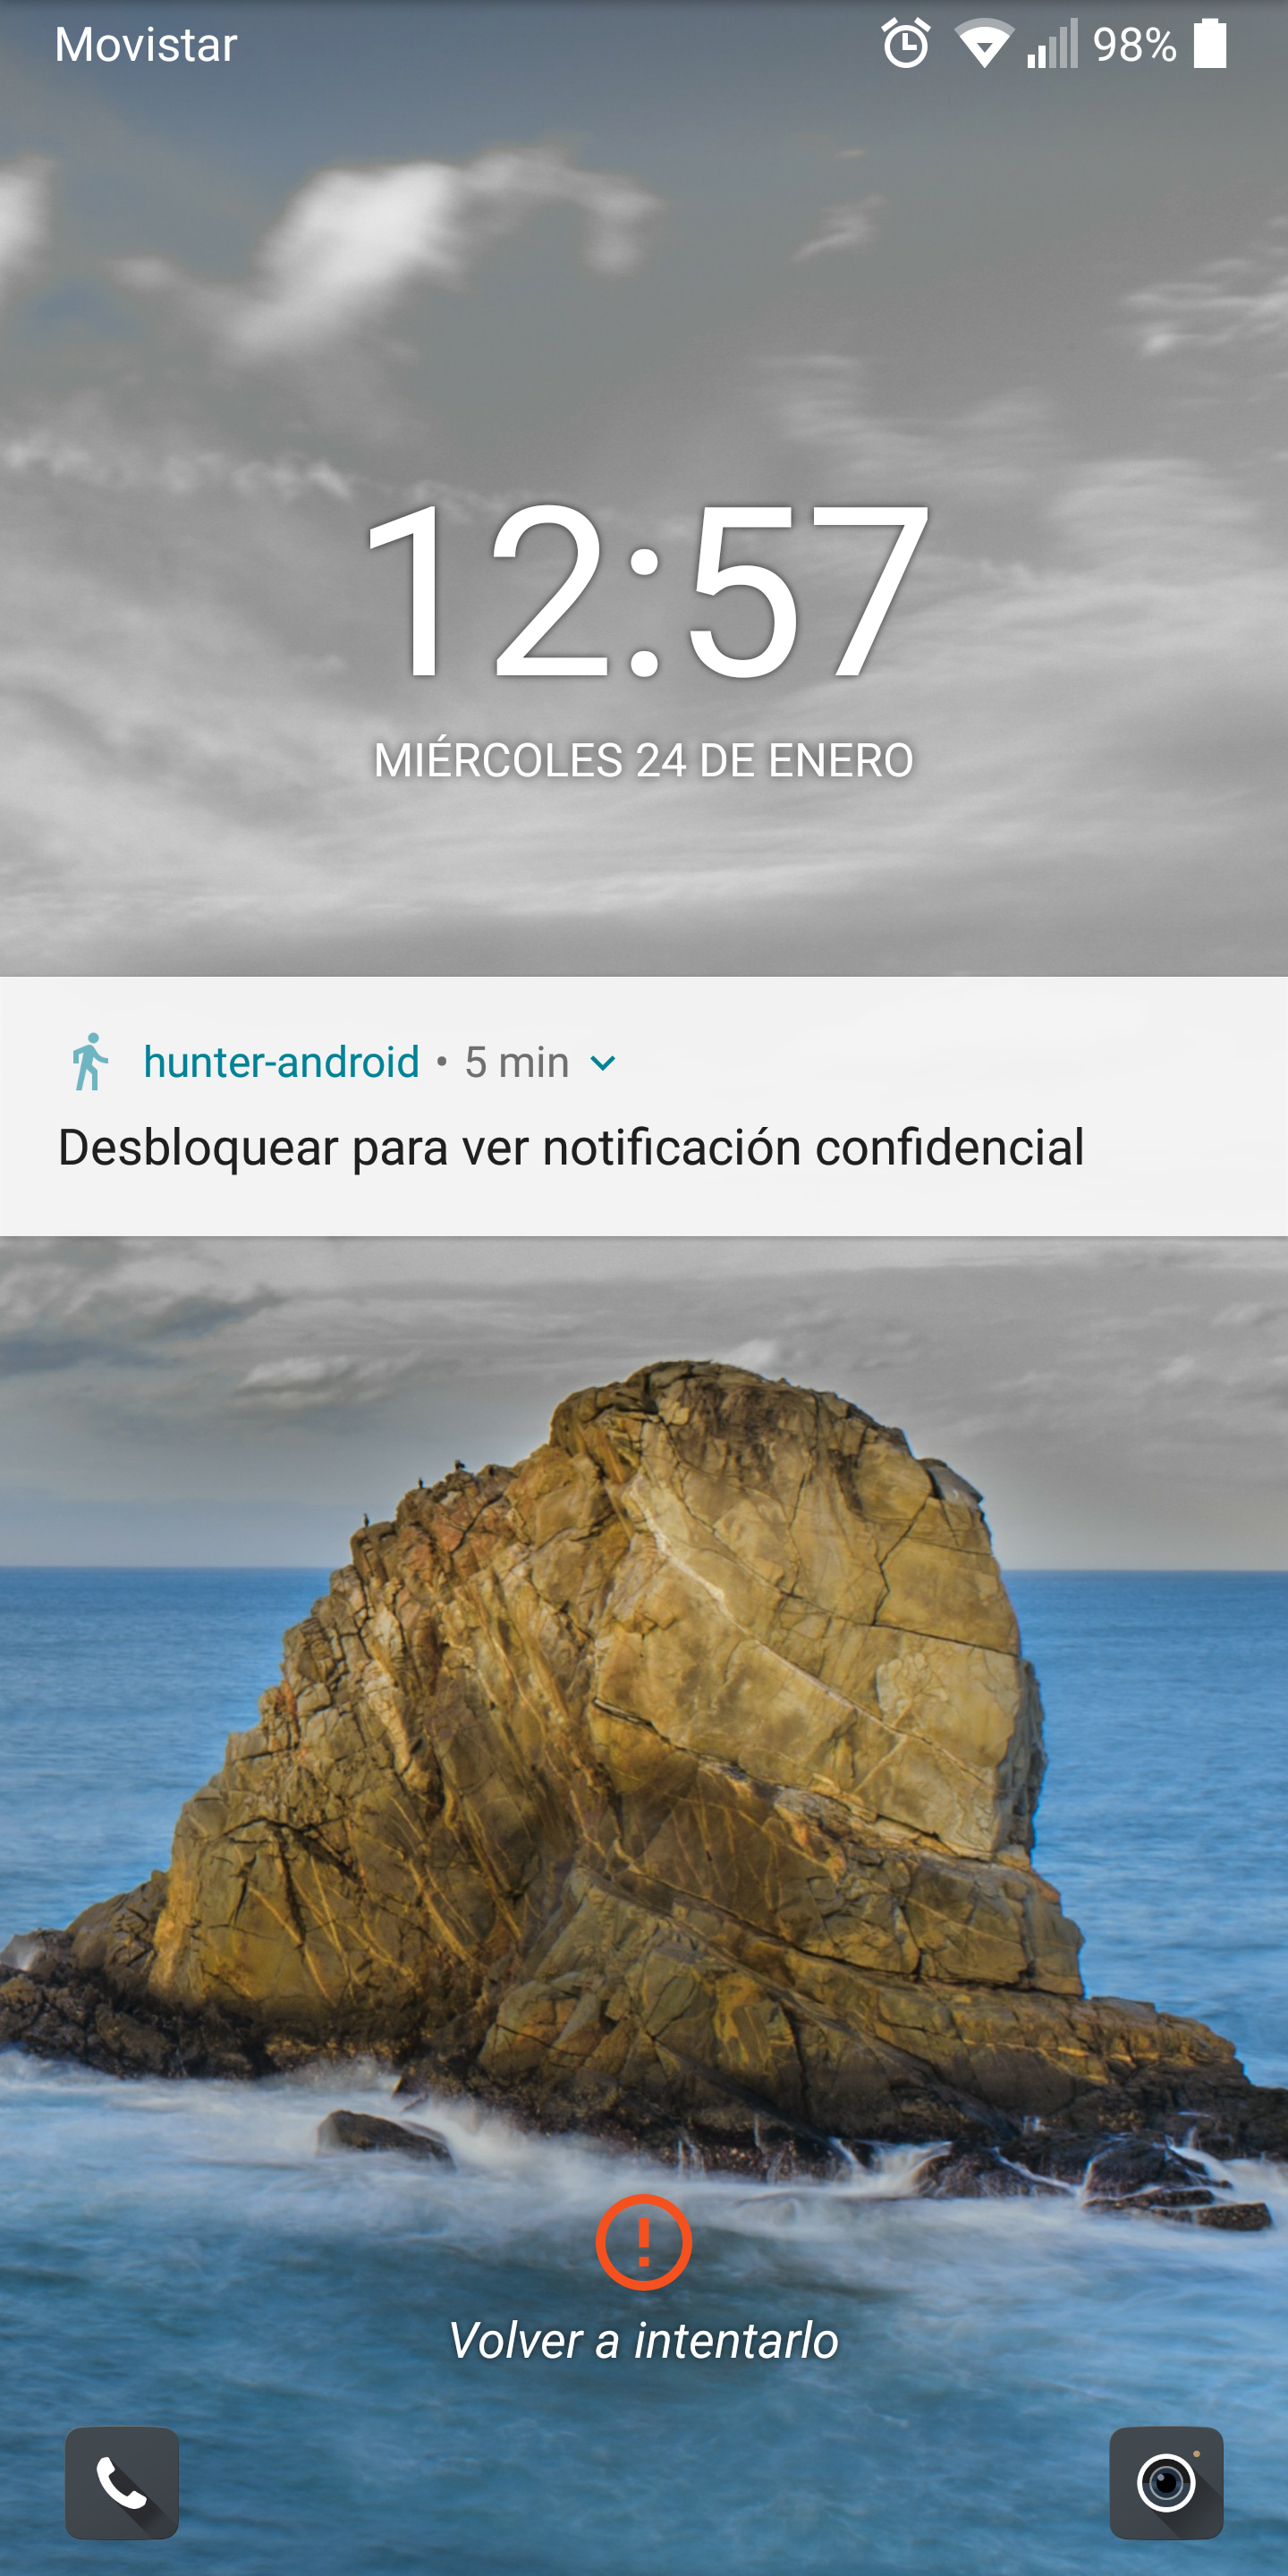
\includegraphics[width=6cm]{capturamovil/push2.png}
 \label{figura2}

\end{minipage}
\caption{Notificación push }
\end{figure} 
 
	
\newpage
	
\section{Pruebas}
Las pruebas son un tema muy importante a tener en cuenta en cualquier proyecto de software. Nos permiten conoces ciertos aspectos que fallan en el sistema de manera objetiva y conocer ciertos riesgos que se nos pasaron por alto en la implementacion.
Dado que usamos la metodología Scrum y como describimos en el capitulo de Seguimiento al final de cada Sprint se harán las pruebas para esas historias de usuario.



\subsection{Pruebas de unidad}
Las pruebas de unidad se  encargan de comprobar el  buen funcionamiento de partes de código. Esta comprobación se realiza normalmente a nivel de clase  asegurándonos que el funcionamiento es el adecuado.\\En nuestro caso las pruebas de unidad se realizaron en el servidor ayudándonos del framework de pruebas JUnit. Como ya se comentó JUniT es una tecnología que ayuda a la ejecución de pruebas integrado en nuestro Eclipse Java EE IDE para la comprobación del funcionamiento de métodos o clases.

Como también se usó el framework Spring para el desarrollo este también fue empleado para los test ya que ayuda a la inyección de dependencias y otras gestiones de las transacciones.



\begin{lstlisting}[language=java,
 ,backgroundcolor=\color{backcolour},   
    commentstyle=\color{codegreen},
    keywordstyle=\color{magenta},
    numberstyle=\tiny\color{codegray},
    stringstyle=\color{codepurple}]
@RunWith(SpringJUnit4ClassRunner.class)
@WebAppConfiguration
@Profile("test")
@ContextConfiguration("classpath:root-context.xml")
public class UsuarioServiceTest {

	@Autowired
	private UsuarioService usuarioService;
	
	@Test
	public void testprueba() {

\end{lstlisting}







\subsection{Pruebas de integración y aceptación}
Las pruebas de integración entre los componentes del sistema y las de aceptación se realizaron de forma manual. En ellas se comprobaba el funcionamiento y la respuesta antes las acciones realizadas.\\
Como el servidor estaba desplegado en un servidor de aplicaciones las pruebas se podían realizar de 2 maneras:
\begin{itemize}
\item Mediante el emulador propio de Android.\\
Esta opción fue la utilizada para depurar la aplicación en los primeros Sprint ya que era más cómodo a la hora realizar las pruebas usar el teclado.
\item  Mediante un móvil en el cual se instalaba nuestra aplicación. En cambio esta opción  fue la más utilizada en los últimos Sprints ya que requerían unas pruebas más reales en  lugares abiertos, ya que se perseguía la comprobación de la precisión del GPS  en casos reales de uso. Esto fue clave para mejora de la creación de rutas.
\end{itemize}










\chapter{Conclusiones y trabajo futuro}
        

\section{Trabajo realizado}
Una vez finalizado este Proyecto de Fin de Grado tenemos una aplicación móvil en Android que cumple todos los objetivos marcados al inicio del proyecto y en especial de esta memoria. La aplicación permitirá al usuario gestionar sus grupos, gestionar sus puntos de interés y guardar sus rutas tantos las que hace de manera individual como las que hace de manera conjunta. Esto último lo hace gracias al sistema de localización del GPS.\\


A continuación se muestran las principales características del producto construido: 

\begin{itemize}
\item Registrarse para poder disfrutar de las funcionalidades que ofrecemos y llevar un seguimiento de sus actuaciones en el campo.
\item Guardar puntos estratégicos en el mapa acompañados de un nombre clave y una breve descripción. Esto nos ayudará a recordar puntos para futuras aventuras. 
\item Crear grupos de compañeros y poder añadirlos para compartir rutas.
\item Guardar las rutas seguidas en nuestras aventuras de pesca y de caza, como también la posibilidad de rememorar esas rutas al poder revisarlas gracias a nuestras lista con las rutas seguidas.
\item Y por último la posibilidad de realizar rutas conjuntas con un grupo de amigos que nosotros queramos y así compartir nuestra ubicación en todo momento. Esto nos ayudará en la pesca ya que al conocer la ubicación del resto de integrantes del grupo podríamos socorrerlo si algo le pasa en un sitio de difícil acceso. Como también por tema de seguridad en una jornada de caza ya que si estamos cerca de otro usuario lo veríamos.
\end{itemize}  

\section{Trabajo futuro}
 La aplicación cumple con los objetivos marcados pero como todo proyecto software puede ser ampliado y mejorado. Una vez finalizado este proyecto, se podrían añadir nuevas funcionalidades:



\begin{itemize}
\item Añadir nuevos tipos de PDIs como es el caso de fotografía. Ya que tiene varias semejanzas con la caza y la pesca por los lugares donde se realiza sería una funcionalidad interesante.
\item Como toda actividad que se realiza al aire libre esta condicionada para bien o para mal por condiciones meteorologías, se podrían usar los servicios de OpenWeatherMap. Esto nos ayudaría a planear mejor nuestras jornadas de pesca, caza o fotografía.


\item Otro punto interesante también sería poder añadir a cada PDI una foto asociada a él, lo que ayudaría a acordarse mejor del lugar y ubicarse con precisión.
\end{itemize}

        

\listoftables
\cleardoublepage

\listoffigures
\cleardoublepage

%%%%%%%%%%%%%%%%%%%%%%%%%%%%%%%%%%%%%%%%
% Apéndices
%%%%%%%%%%%%%%%%%%%%%%%%%%%%%%%%%%%%%%%%
\appendix
\addcontentsline{toc}{chapter}{Apéndices}

\chapter{Glosario}
		\label{glosario}
		
\renewcommand*{\arraystretch}{1.5}
\begin{description}
\item{





\end{description}
		\cleardoublepage

\cleardoublepage


%%%%%%%%%%%%%%%%%%%%%%%%%%%%%%%%%%%%%%%%
% Bibliografía
%%%%%%%%%%%%%%%%%%%%%%%%%%%%%%%%%%%%%%%%
\bibliographystyle{alpha}
\bibliography{references}
\end{document}


